\documentclass[11pt]{beamer}
\usepackage{ctex, hyperref}
\usepackage[T1]{fontenc}

% other packages
\usepackage{latexsym,amsmath,xcolor,multicol,booktabs,calligra}
\usepackage{graphicx,pstricks,listings,stackengine}

\author{讲述人:郭佳明}
\title{ 一个基于LKM的Linux内核级rootkit的实现 }
\subtitle{软件安全原理第三组课程汇报}
\institute{中国科学院信息工程研究所}
\date{2022年10月26日}
\usepackage{PekingU}

% defs
\def\cmd#1{\texttt{\color{red}\footnotesize $\backslash$#1}}
\def\env#1{\texttt{\color{blue}\footnotesize #1}}
\definecolor{deepblue}{rgb}{0,0,0.5}
\definecolor{deepred}{rgb}{0.6,0,0}
\definecolor{deepgreen}{rgb}{0,0.5,0}
\definecolor{halfgray}{gray}{0.55}

\lstset{
    basicstyle=\ttfamily\small,
    keywordstyle=\bfseries\color{deepblue},
    emphstyle=\ttfamily\color{deepred},    % Custom highlighting style
    stringstyle=\color{deepgreen},
    numbers=left,
    numberstyle=\small\color{halfgray},
    rulesepcolor=\color{red!20!green!20!blue!20},
    frame=shadowbox,
}


\begin{document}

\kaishu
\begin{frame}
    \titlepage
    \begin{figure}[htpb]
        \begin{center}
            
\includegraphics[width=0.2\linewidth]{pic/cas_logo.png}
        \end{center}
    \end{figure}
\end{frame}




%==================显示目录


\begin{frame}%配置参数信息
    \tableofcontents[sectionstyle=show,subsectionstyle=show/shaded/hide,subsubsectionstyle=show/shaded/hide]
\end{frame}




%==================== overview 

\section{Overview}
\subsection{rootkit简介}
\begin{frame}
    \begin{itemize}
        \item 特点
        \begin{itemize}
        	\item 具有隐蔽性
        	\item 提供后门保持root权限访问
        	\item 与内核版本强相关
        \end{itemize}
        \item 分类
        \begin{itemize}
        	\item Linux/Windows
        	\item 内核级(Ring3)/用户级(Ring0)
        \end{itemize}
        \item LKM实现rootkit
        \begin{itemize}
            \item LKM:Loadable Kernel Module(.ko)
            \item 不必重新编译内核,动态加载
        \end{itemize}
    \end{itemize}
\end{frame}

\subsection{一个简单的LKM示例}
\begin{frame}
	\begin{itemize}
		\item insmod加载,rmmod卸载,lsmod显示所有模块
	\end{itemize}
	\begin{itemize}
		\centering
		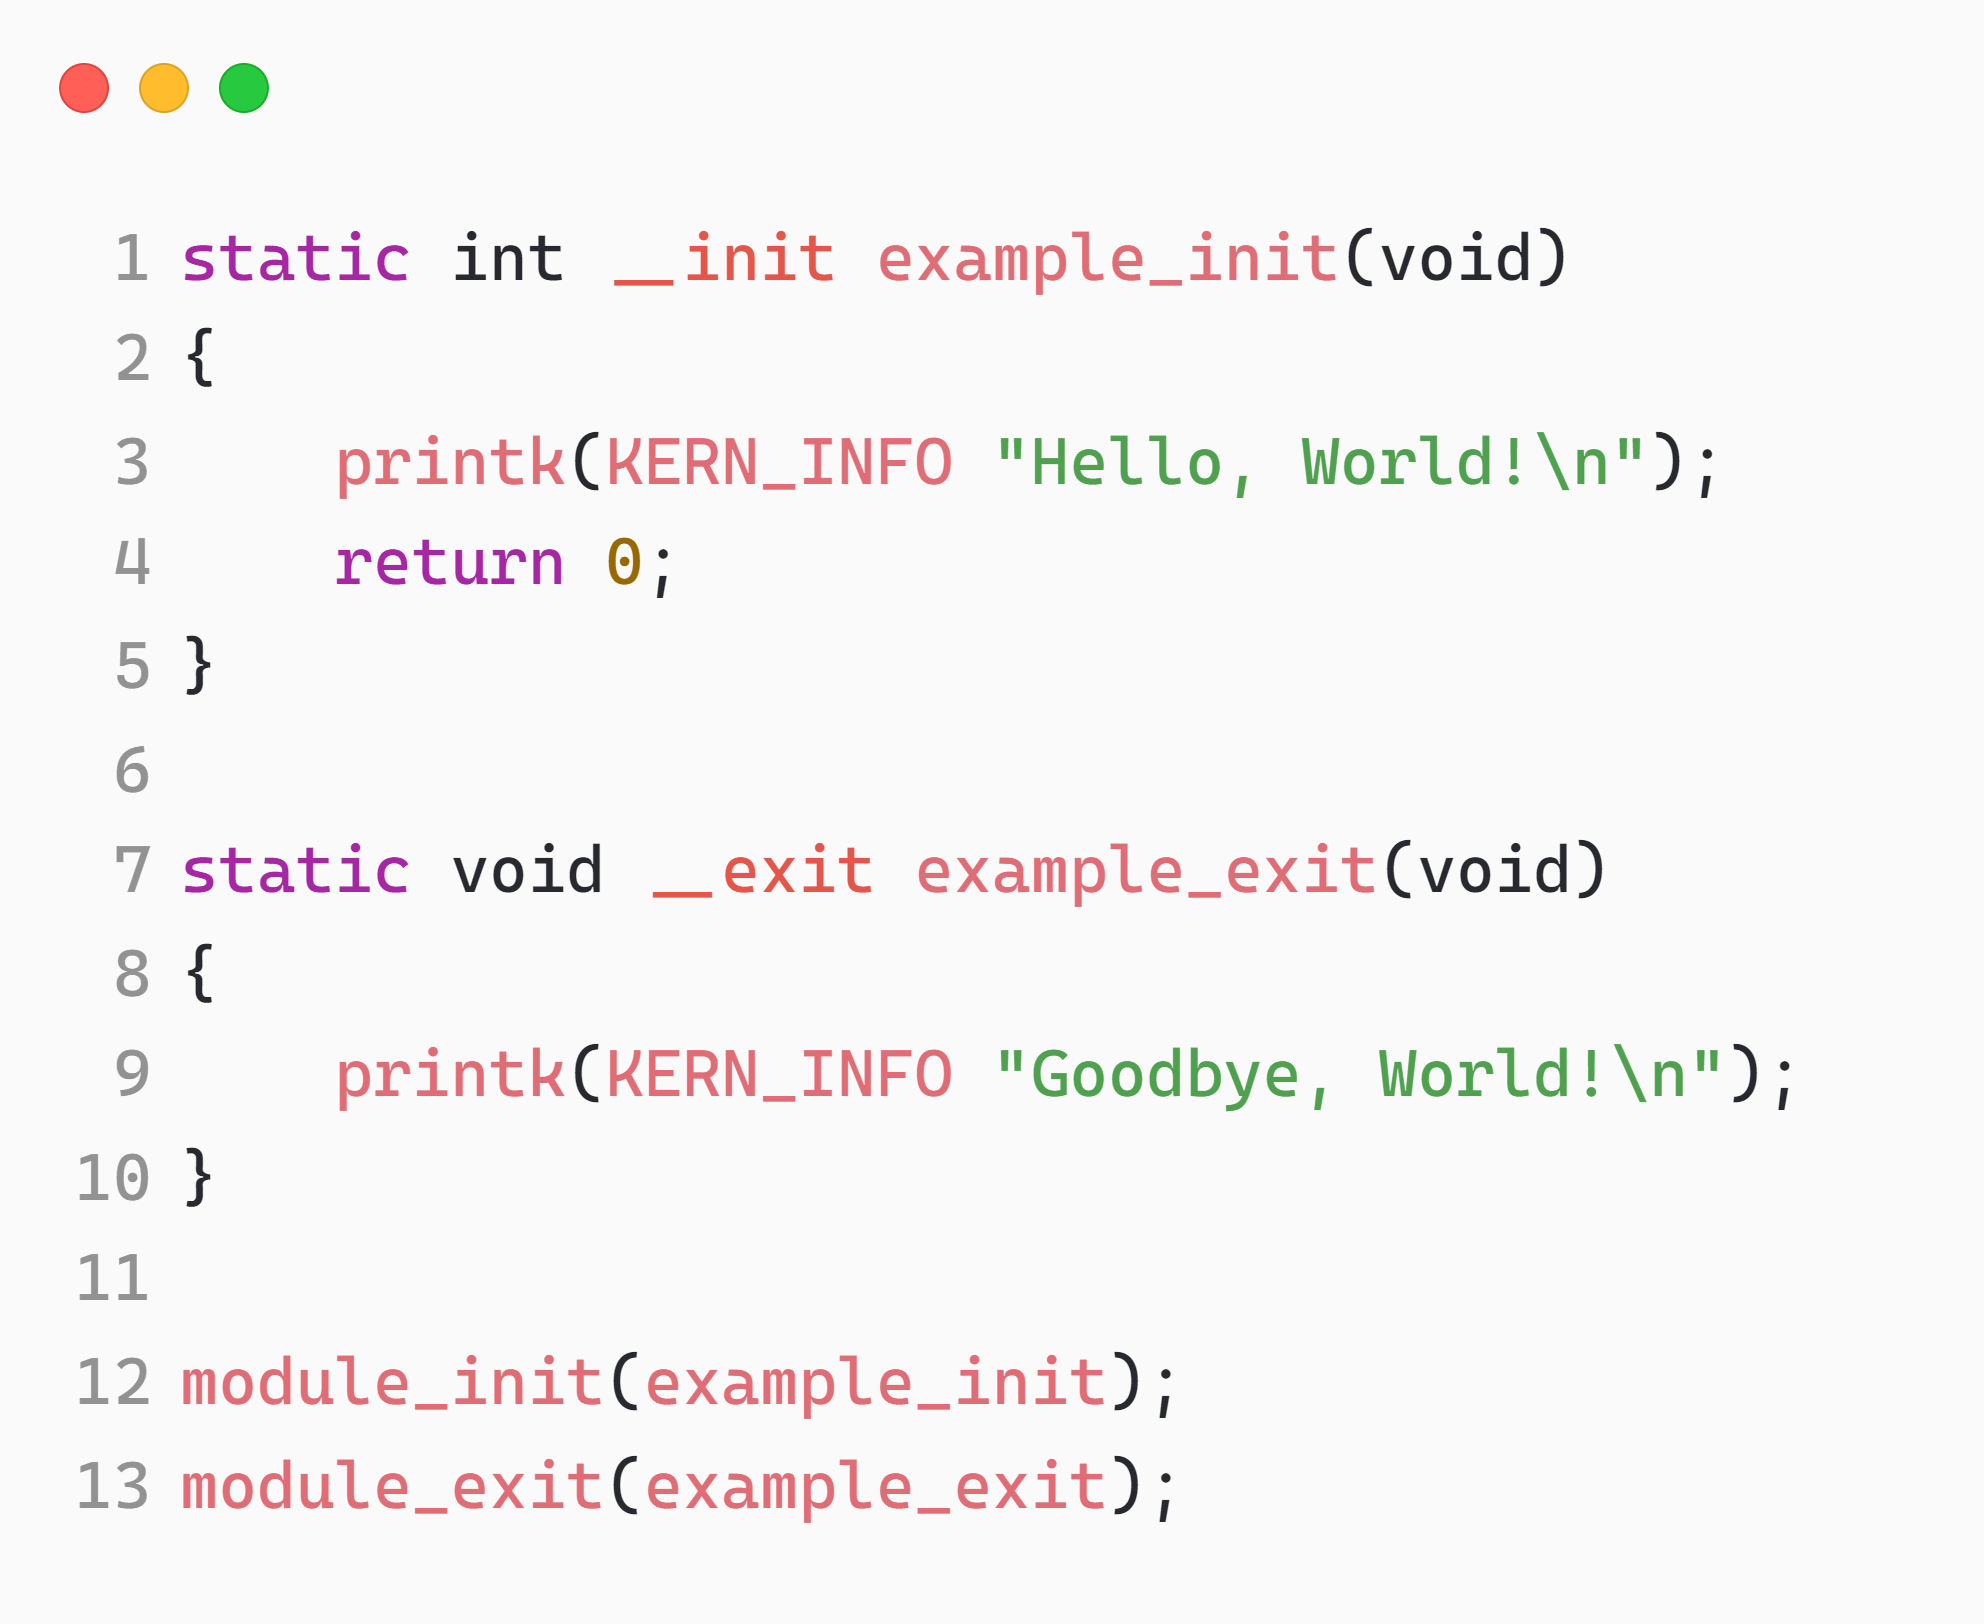
\includegraphics[width=0.80\textwidth]{pic/lkm-demo.png}
	\end{itemize}
	
\end{frame}

\subsection{hook系统调用}
\begin{frame}
	\begin{itemize}
		\item 用户进程使用系统调用陷入内核请求各种服务
		\item hook:劫持系统调用,让内核执行我们自行设计的函数
		\item 系统调用表:存放了所有系统调用的地址
	\end{itemize}
	\begin{itemize}
		\centering
		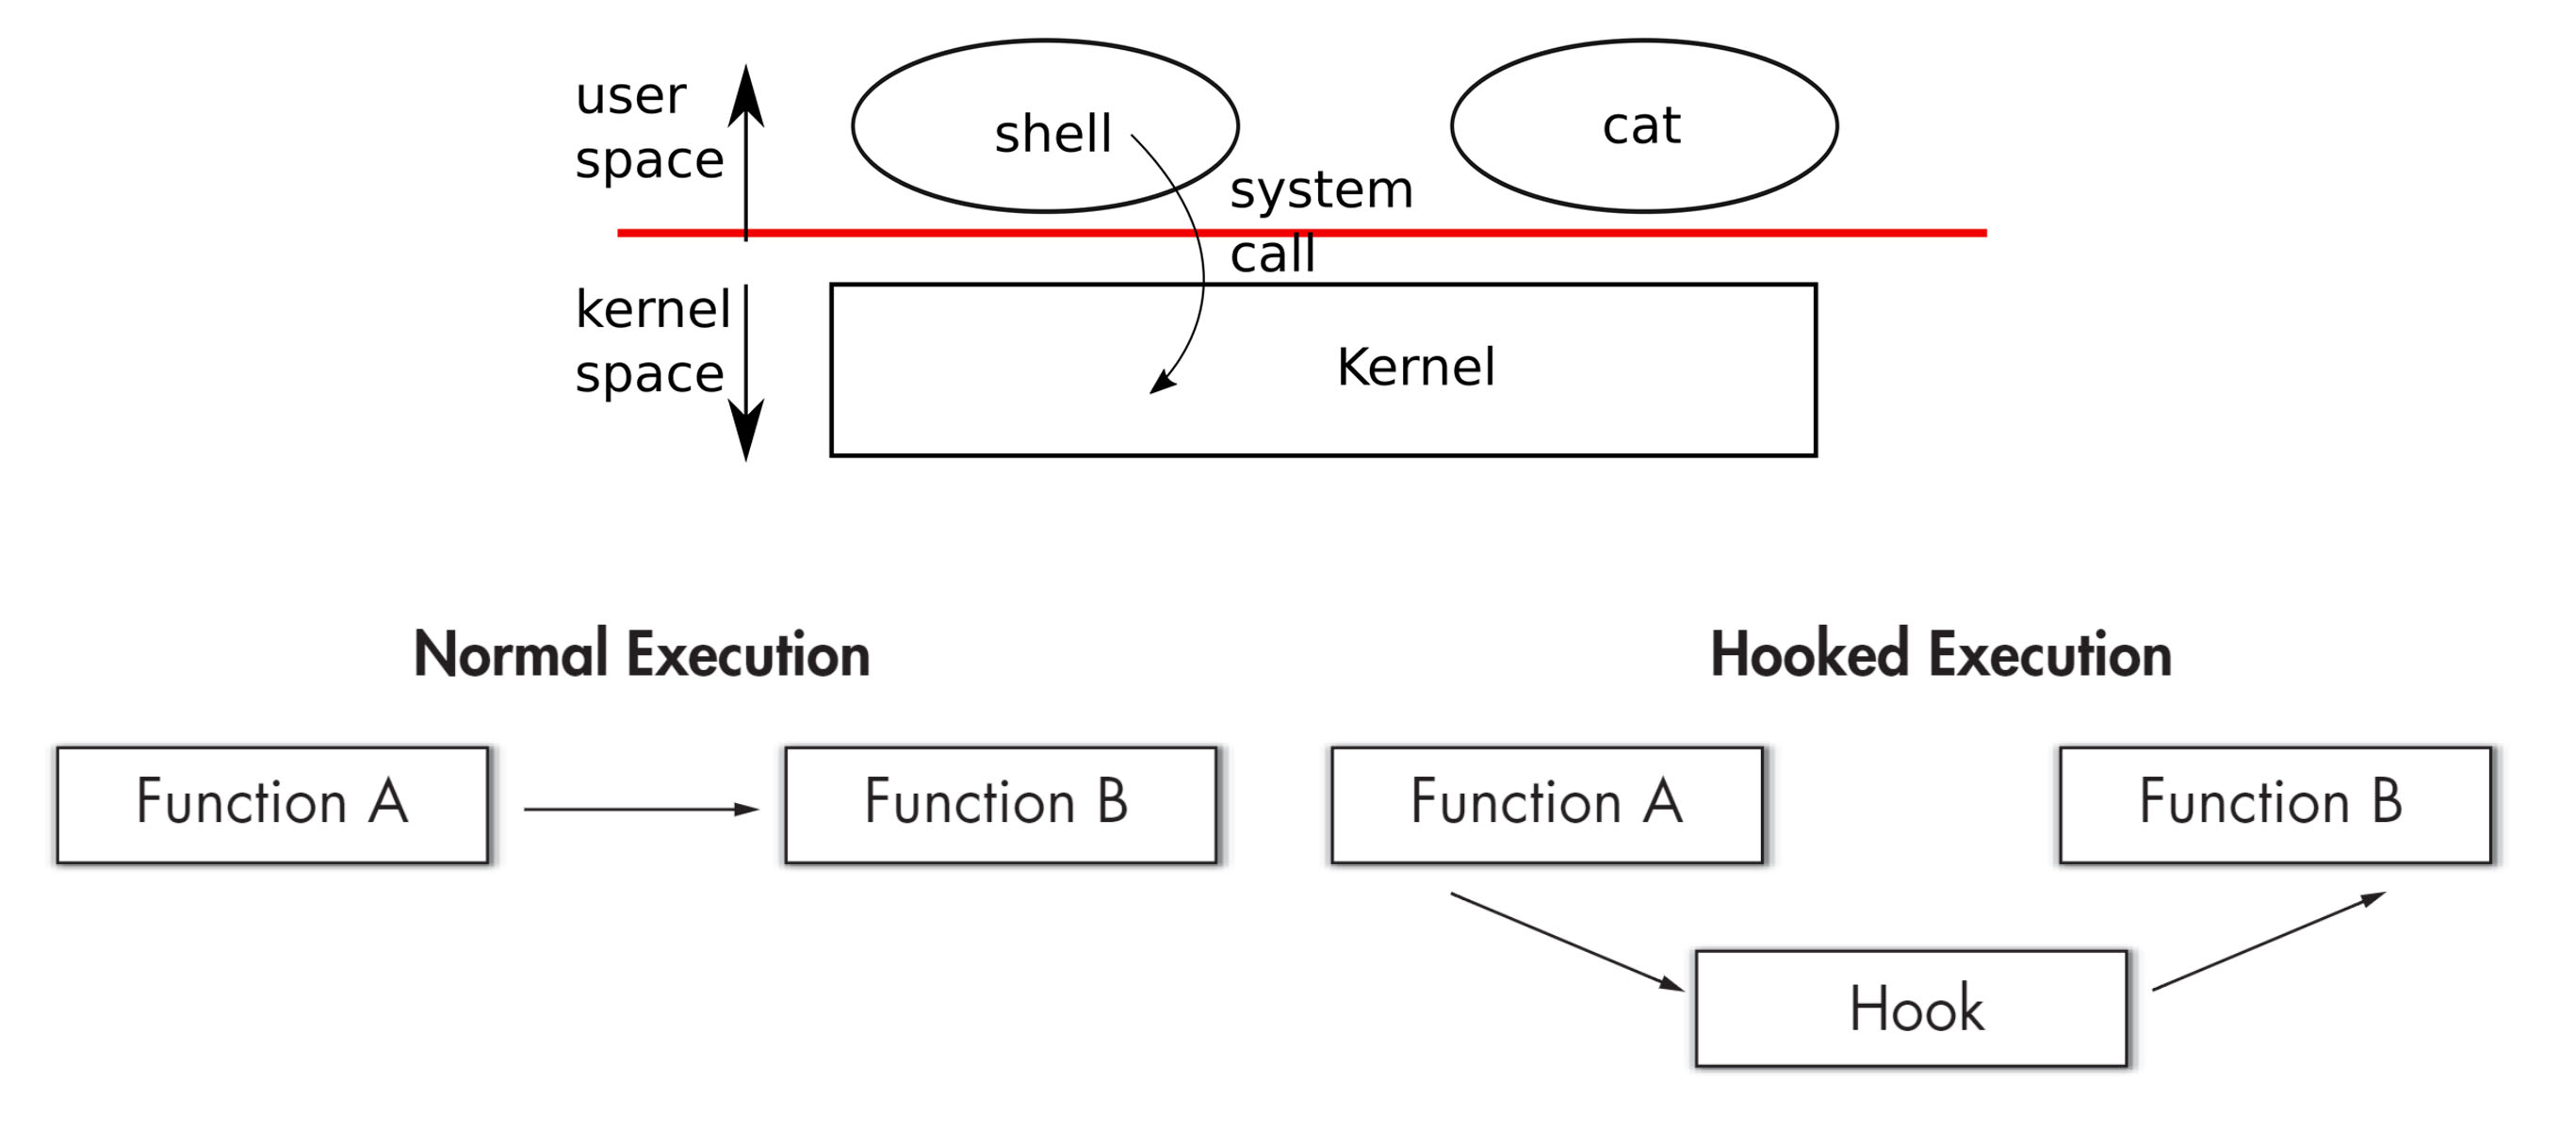
\includegraphics[width=0.85\textwidth]{pic/syscall&hook.jpg}
	\end{itemize}
\end{frame}

\begin{frame}{使用kallsyms获取系统调用表}
	cat /proc/kallsyms | grep xxx
	\begin{itemize}
		\centering
		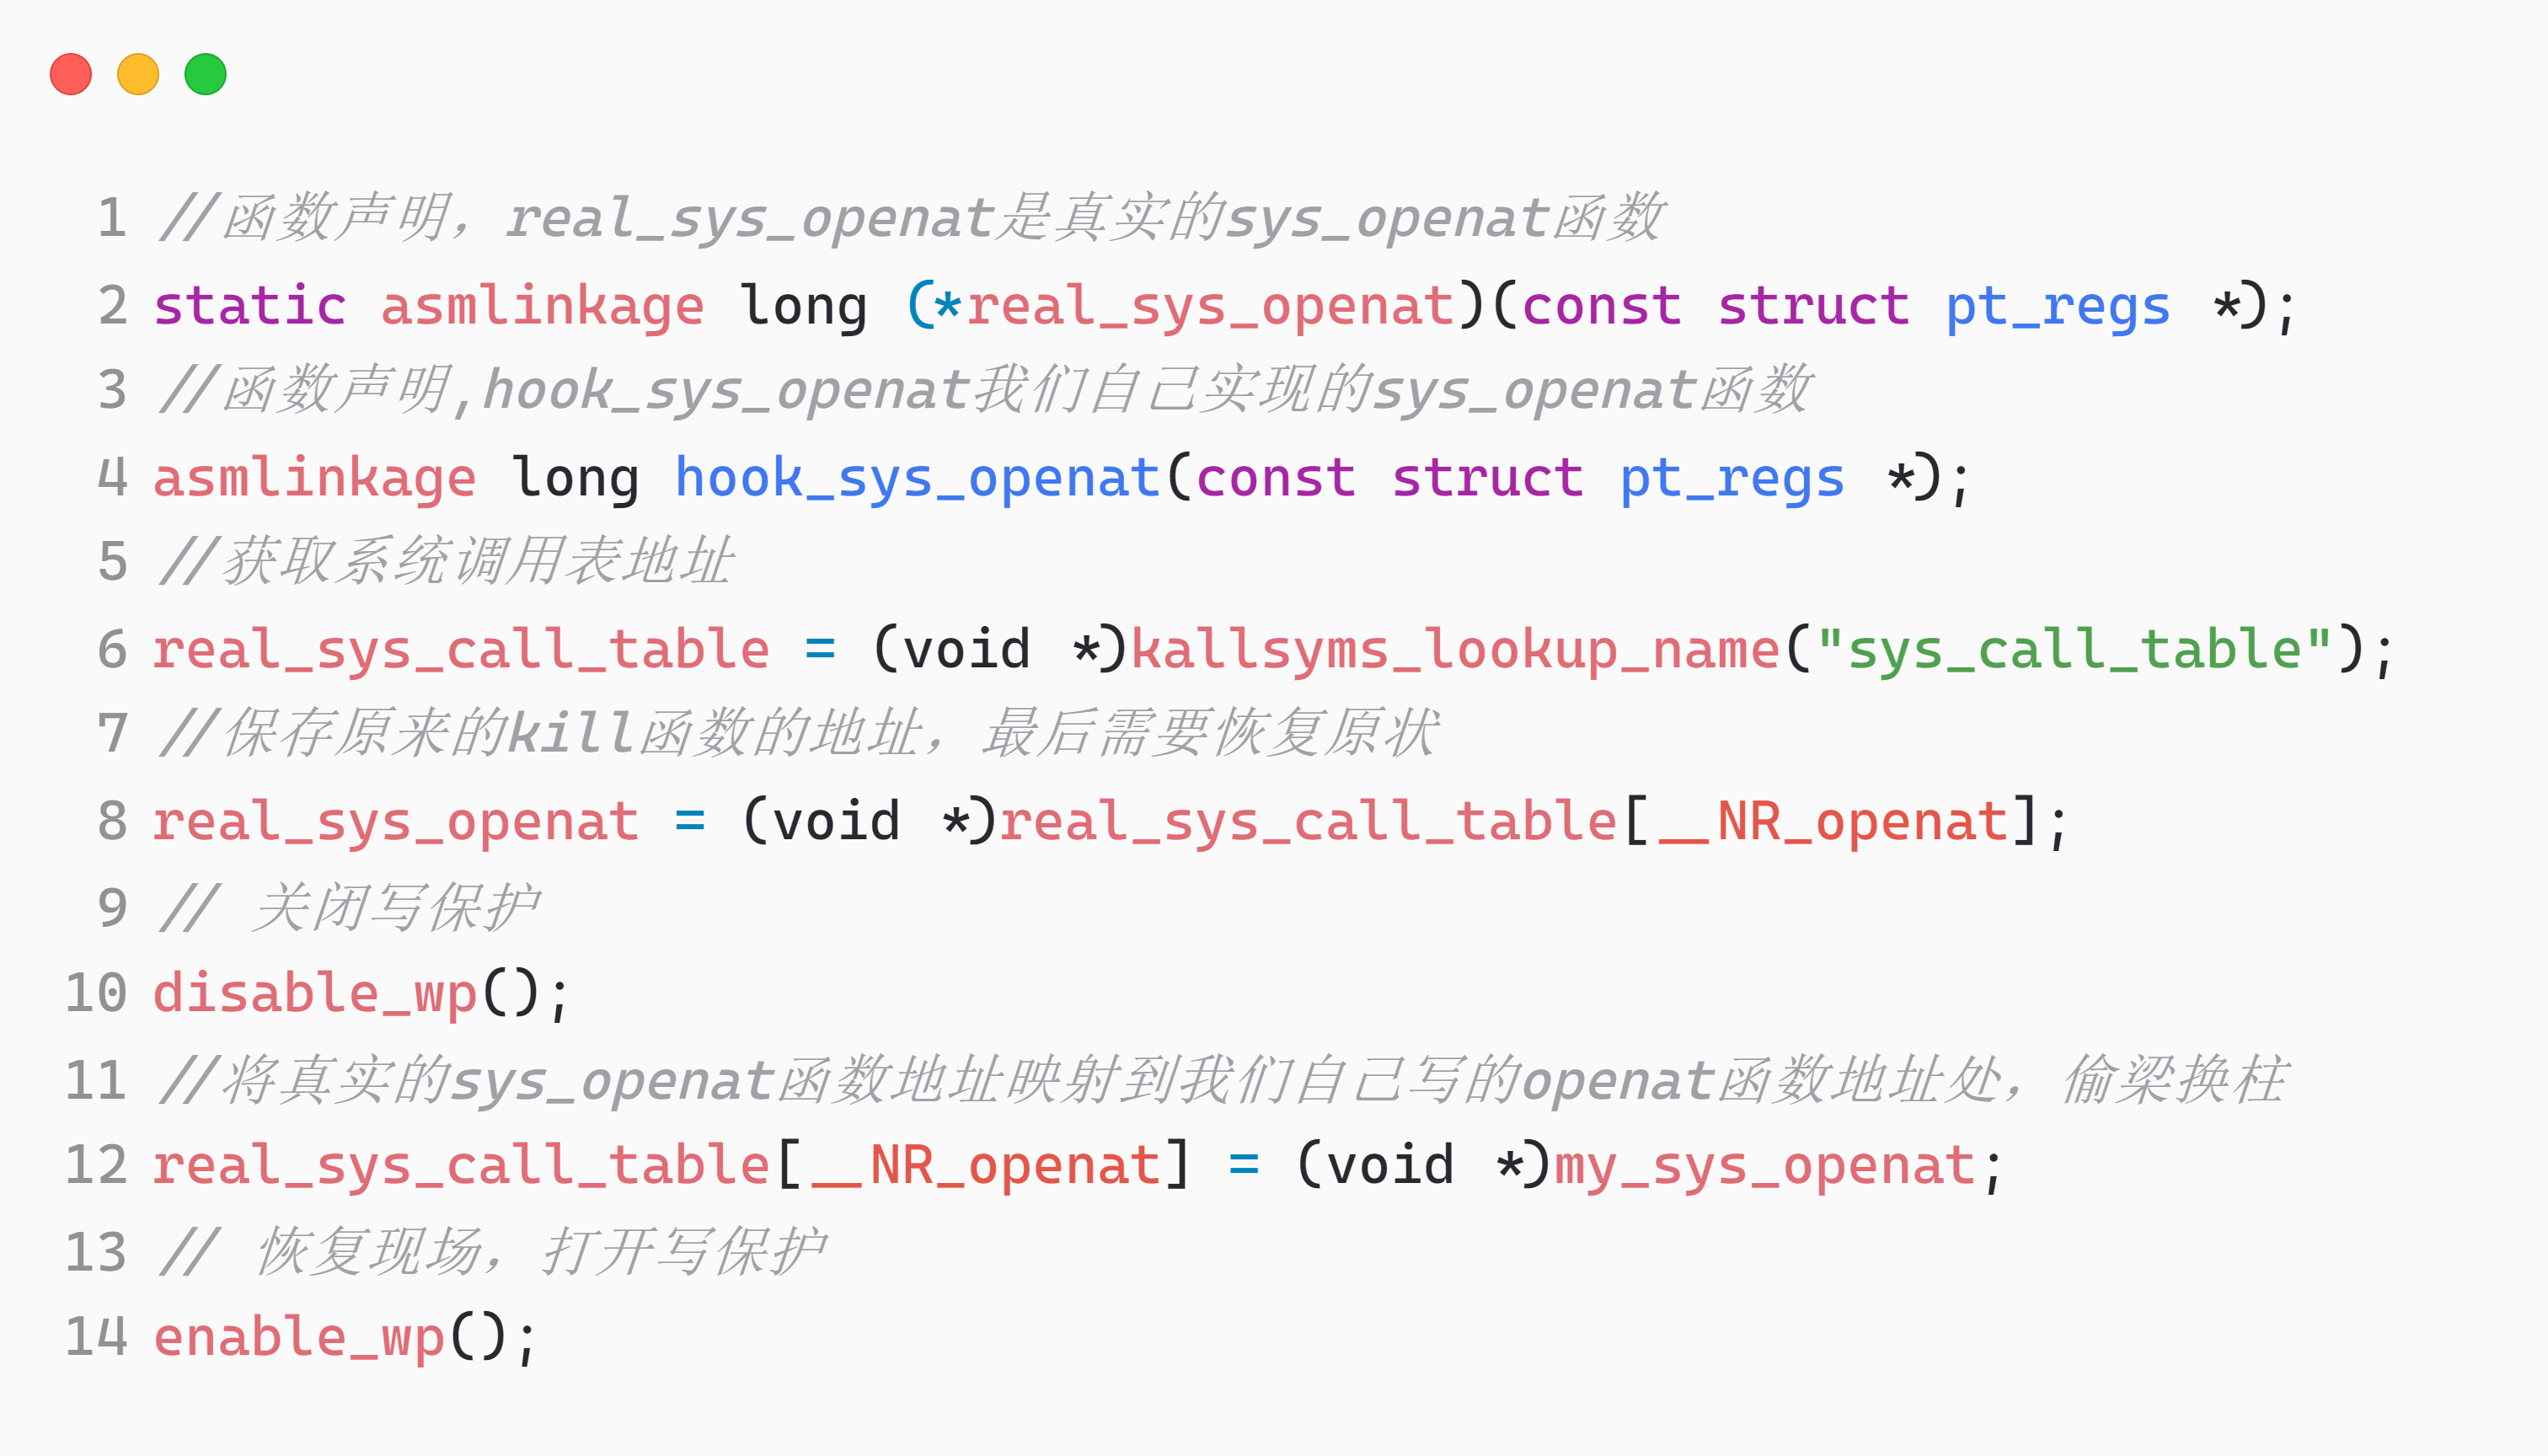
\includegraphics[width=0.95\textwidth]{pic/kallsyms.png}
	\end{itemize}
\end{frame}

\begin{frame}{使用ftrace获取系统调用表}
	\begin{itemize}
		\centering
		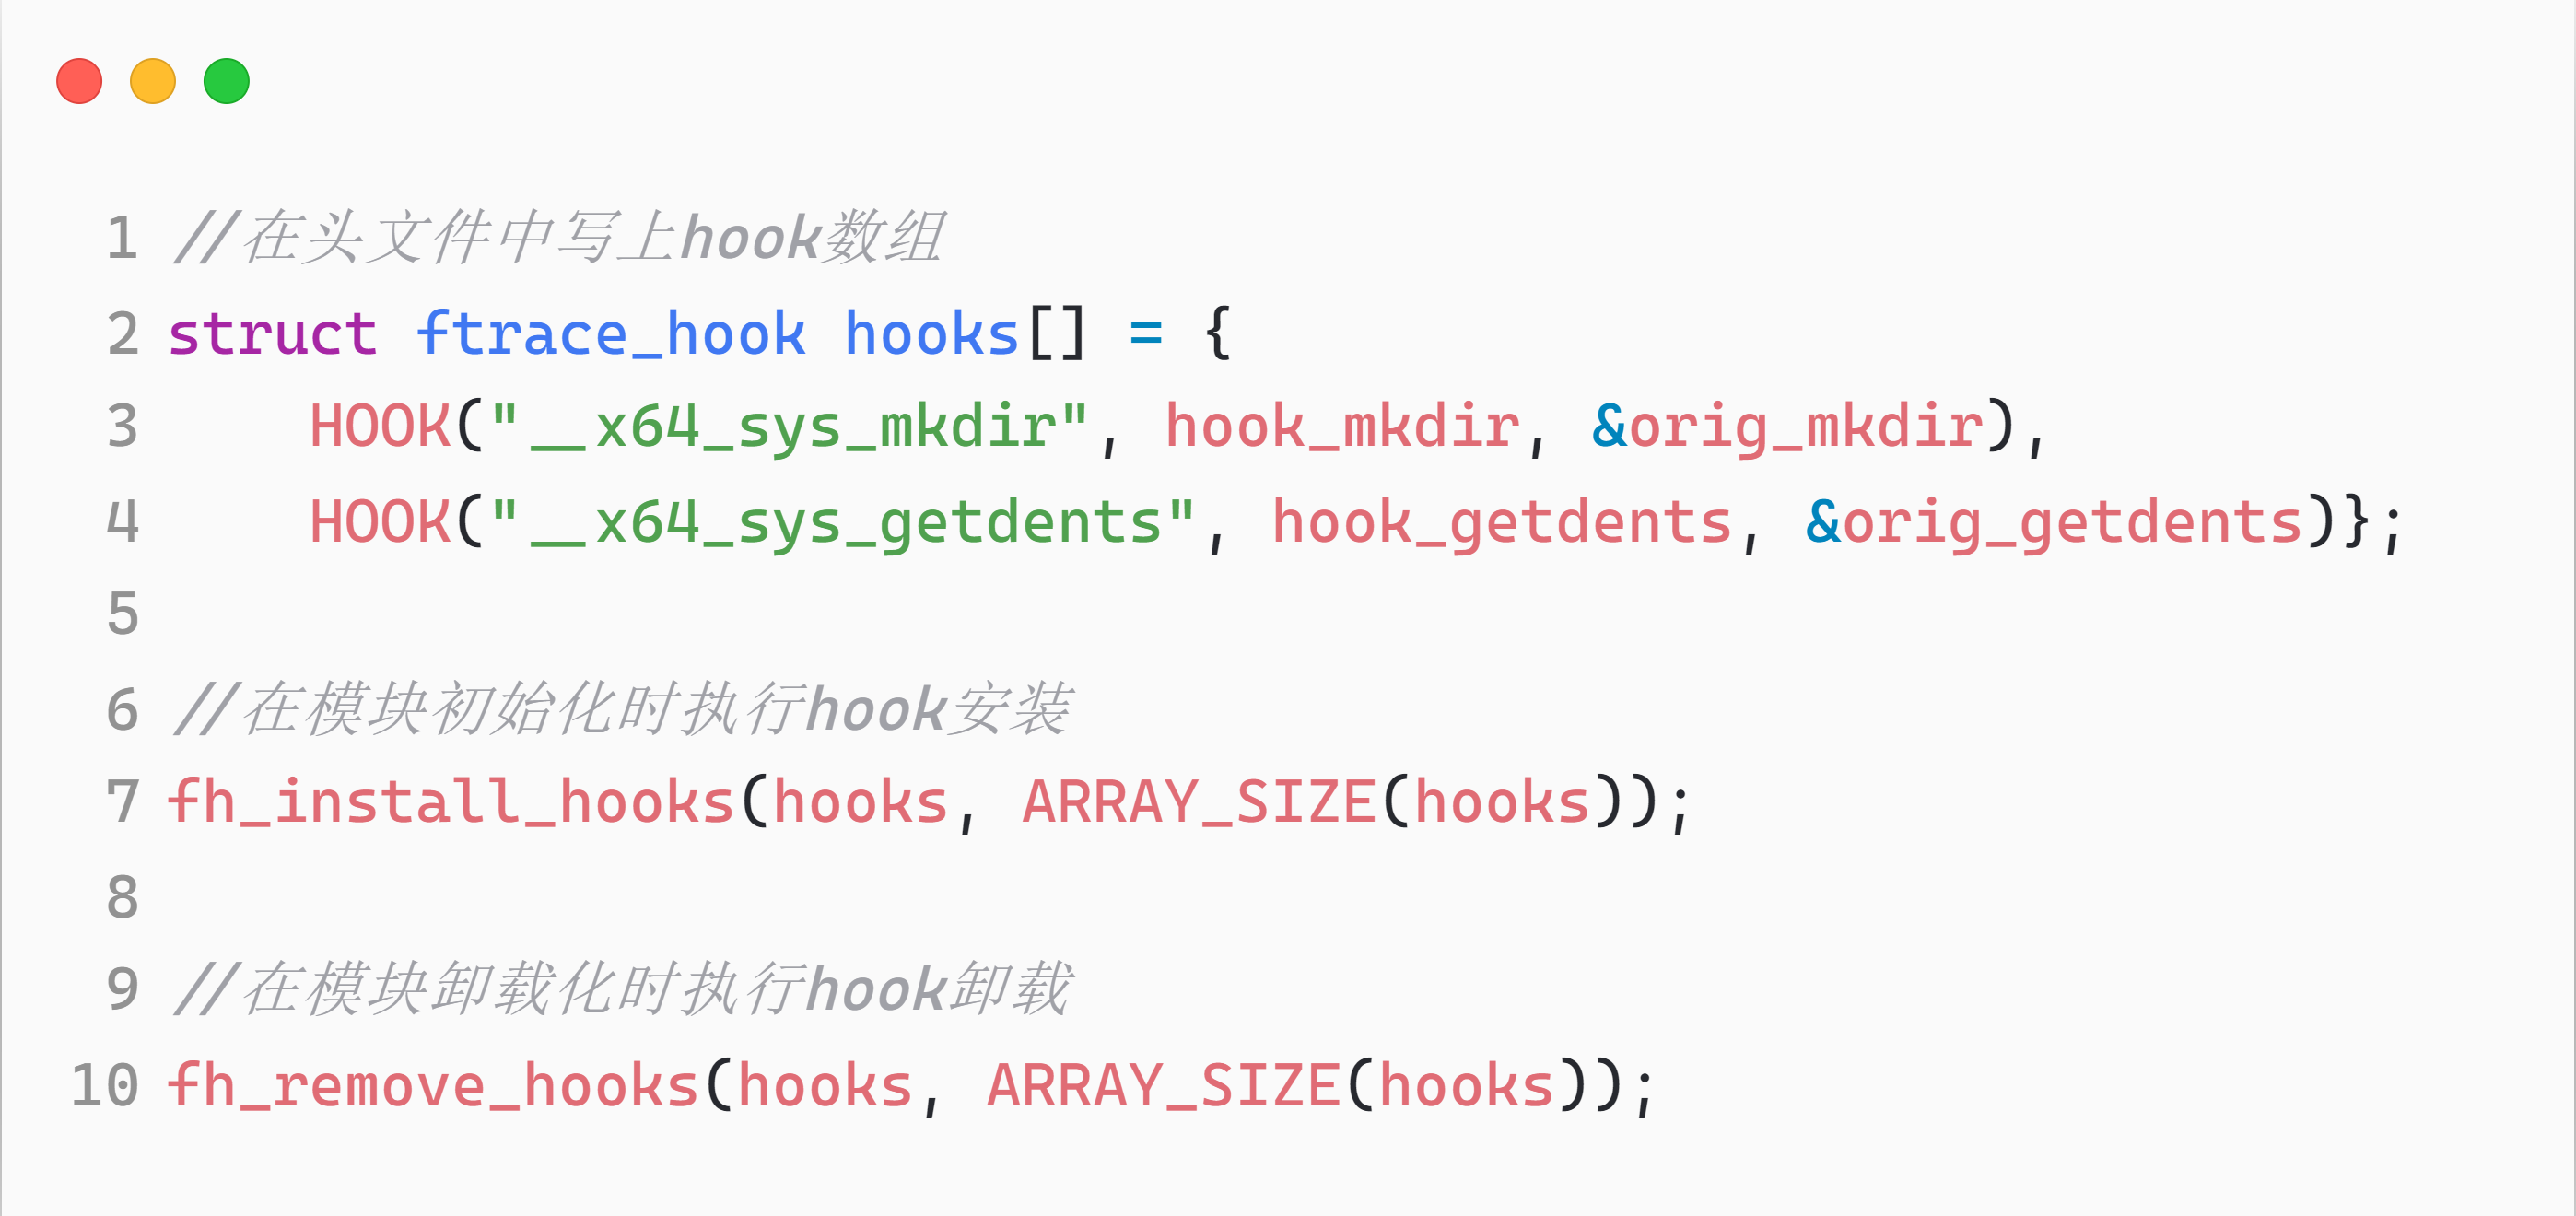
\includegraphics[width=0.95\textwidth]{pic/ftrace.png}
	\end{itemize}
\end{frame}

\begin{frame}{新旧系统调用声明}
	\begin{itemize}
		\item 用户程序下陷到内核态参数的信息都被保存在堆栈
		\item asmlinkage宏:让编译器在 CPU 堆栈上查找函数参数,而不是寄存器
		\item 存储在寄存器中的参数会先被复制到pt\_regs结构体
		\item copy\_from\_user提供用户和内核的数据传输
	\end{itemize}
	\begin{itemize}
		\centering
		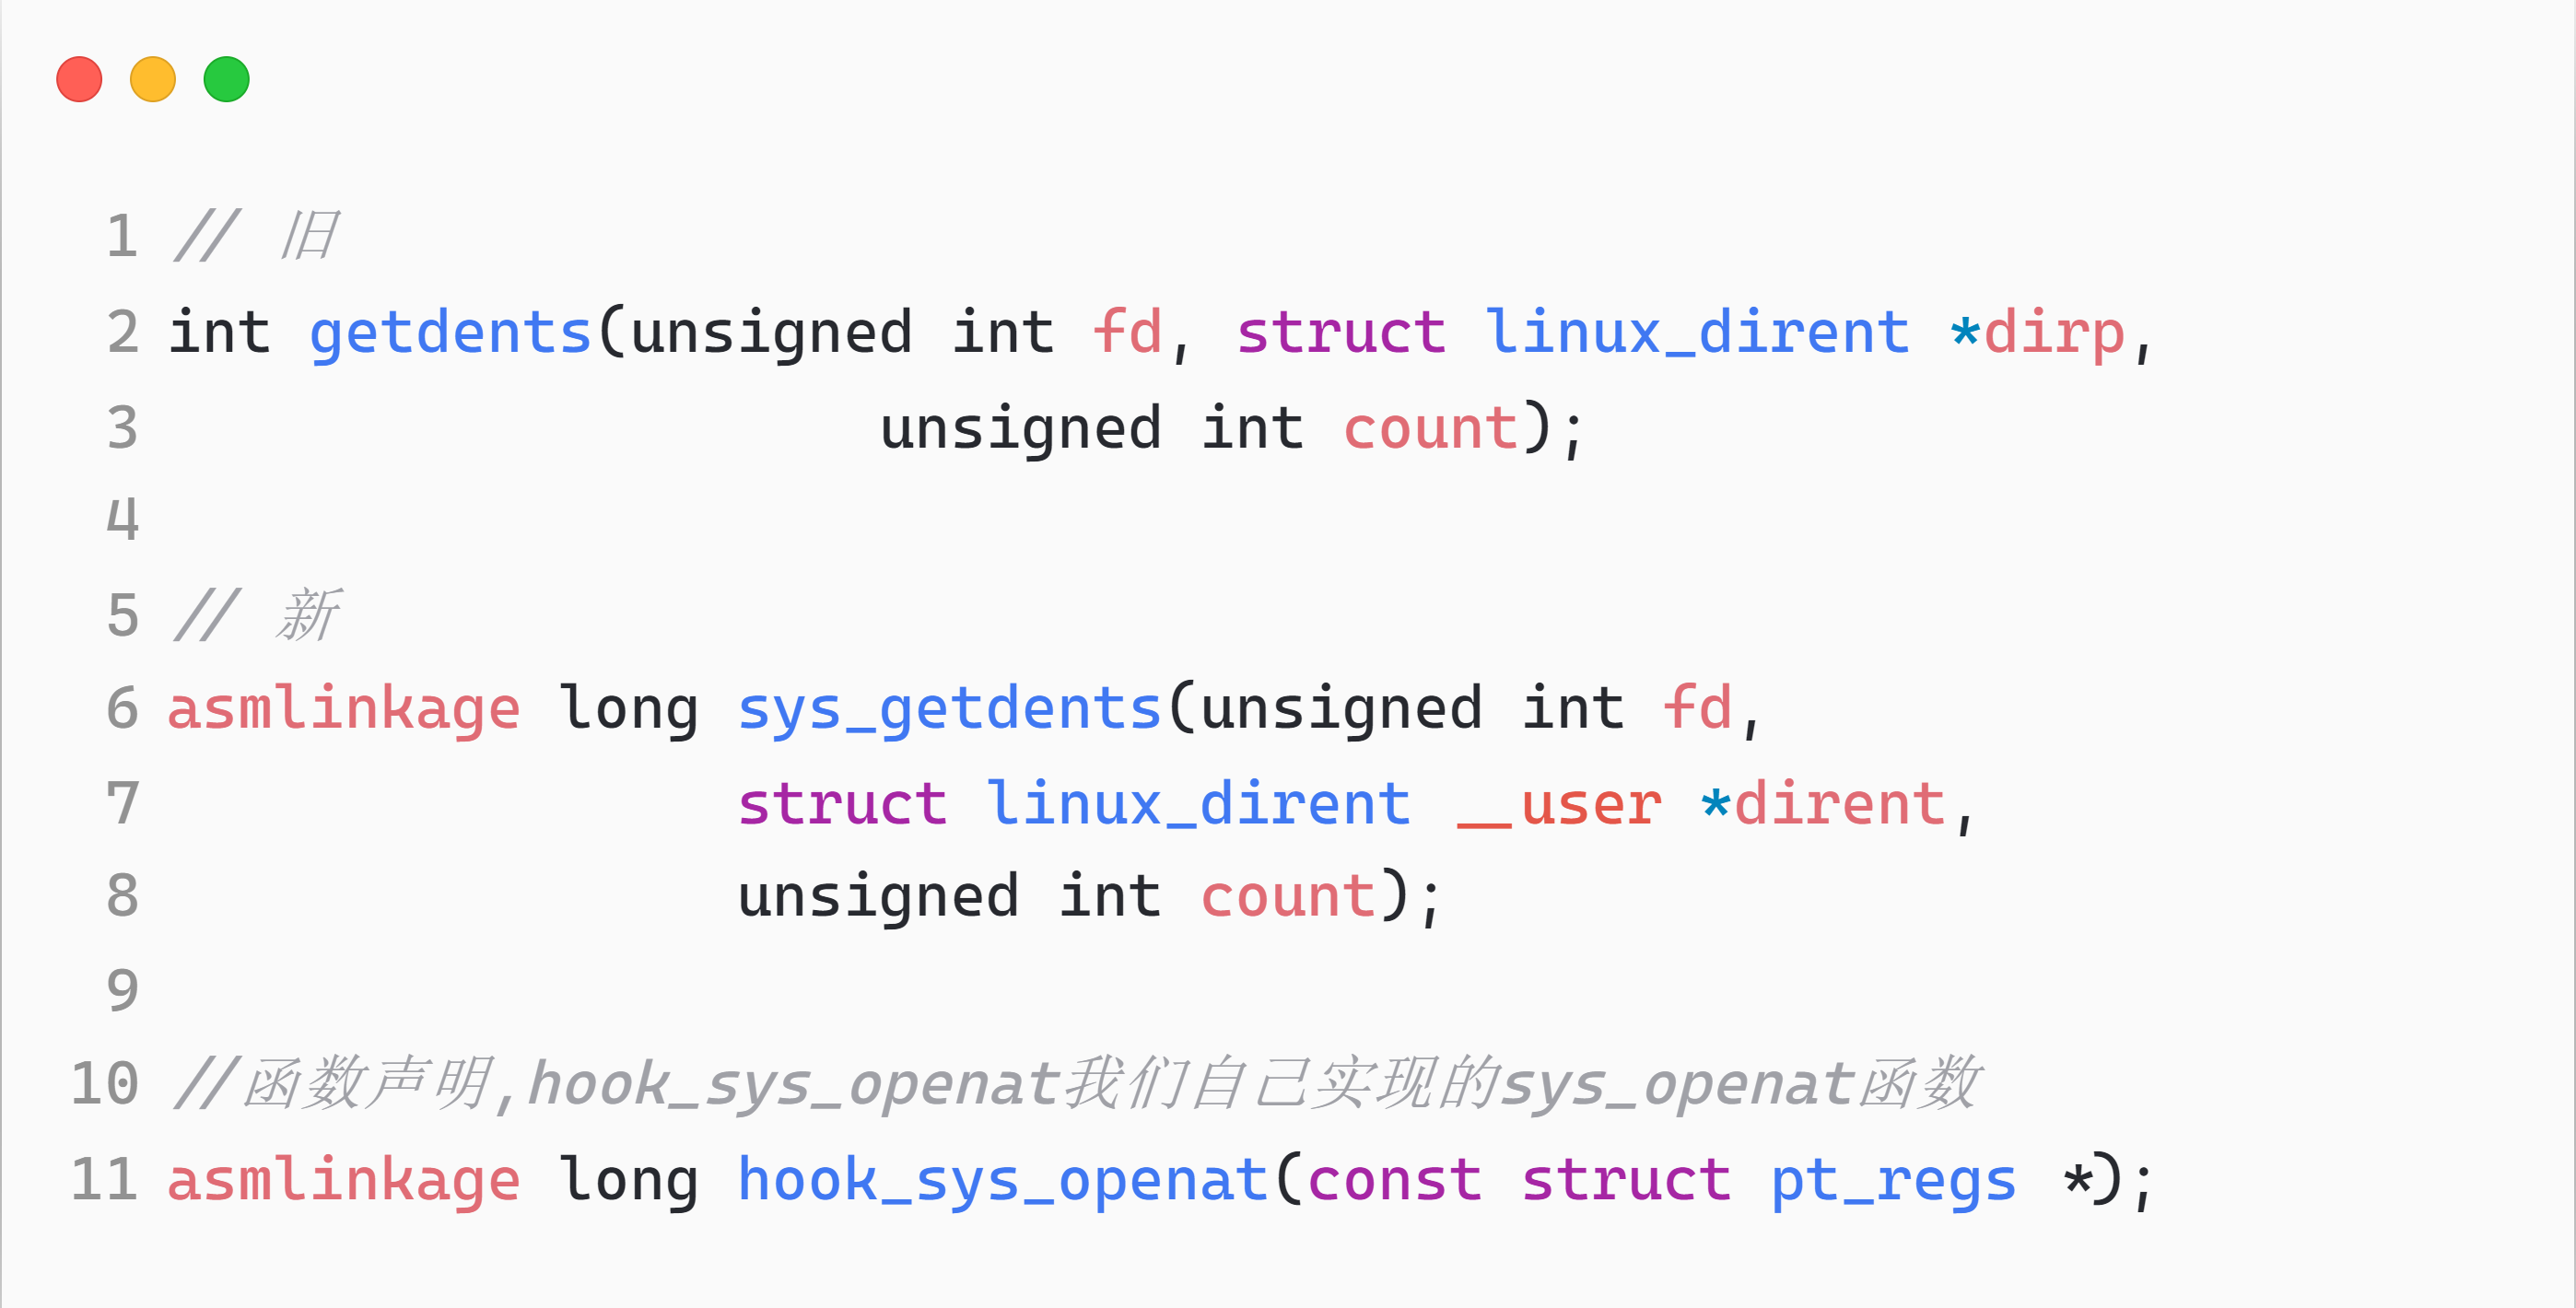
\includegraphics[width=0.80\textwidth]{pic/diff-syscall.png}
	\end{itemize}
\end{frame}


\begin{frame}{开发环境与工具}
	\begin{itemize}
		\item vscode ssh remote + VMware Ubuntu 20.04LTS虚拟机
		\item strace 命令帮助分析函数调用
		\item souce insight阅读内核代码
		\item GitHub实现团队合作
		\item doxygen部署文档
	\end{itemize}
\end{frame}

\begin{frame}{strace}
		\begin{itemize}
			\centering
			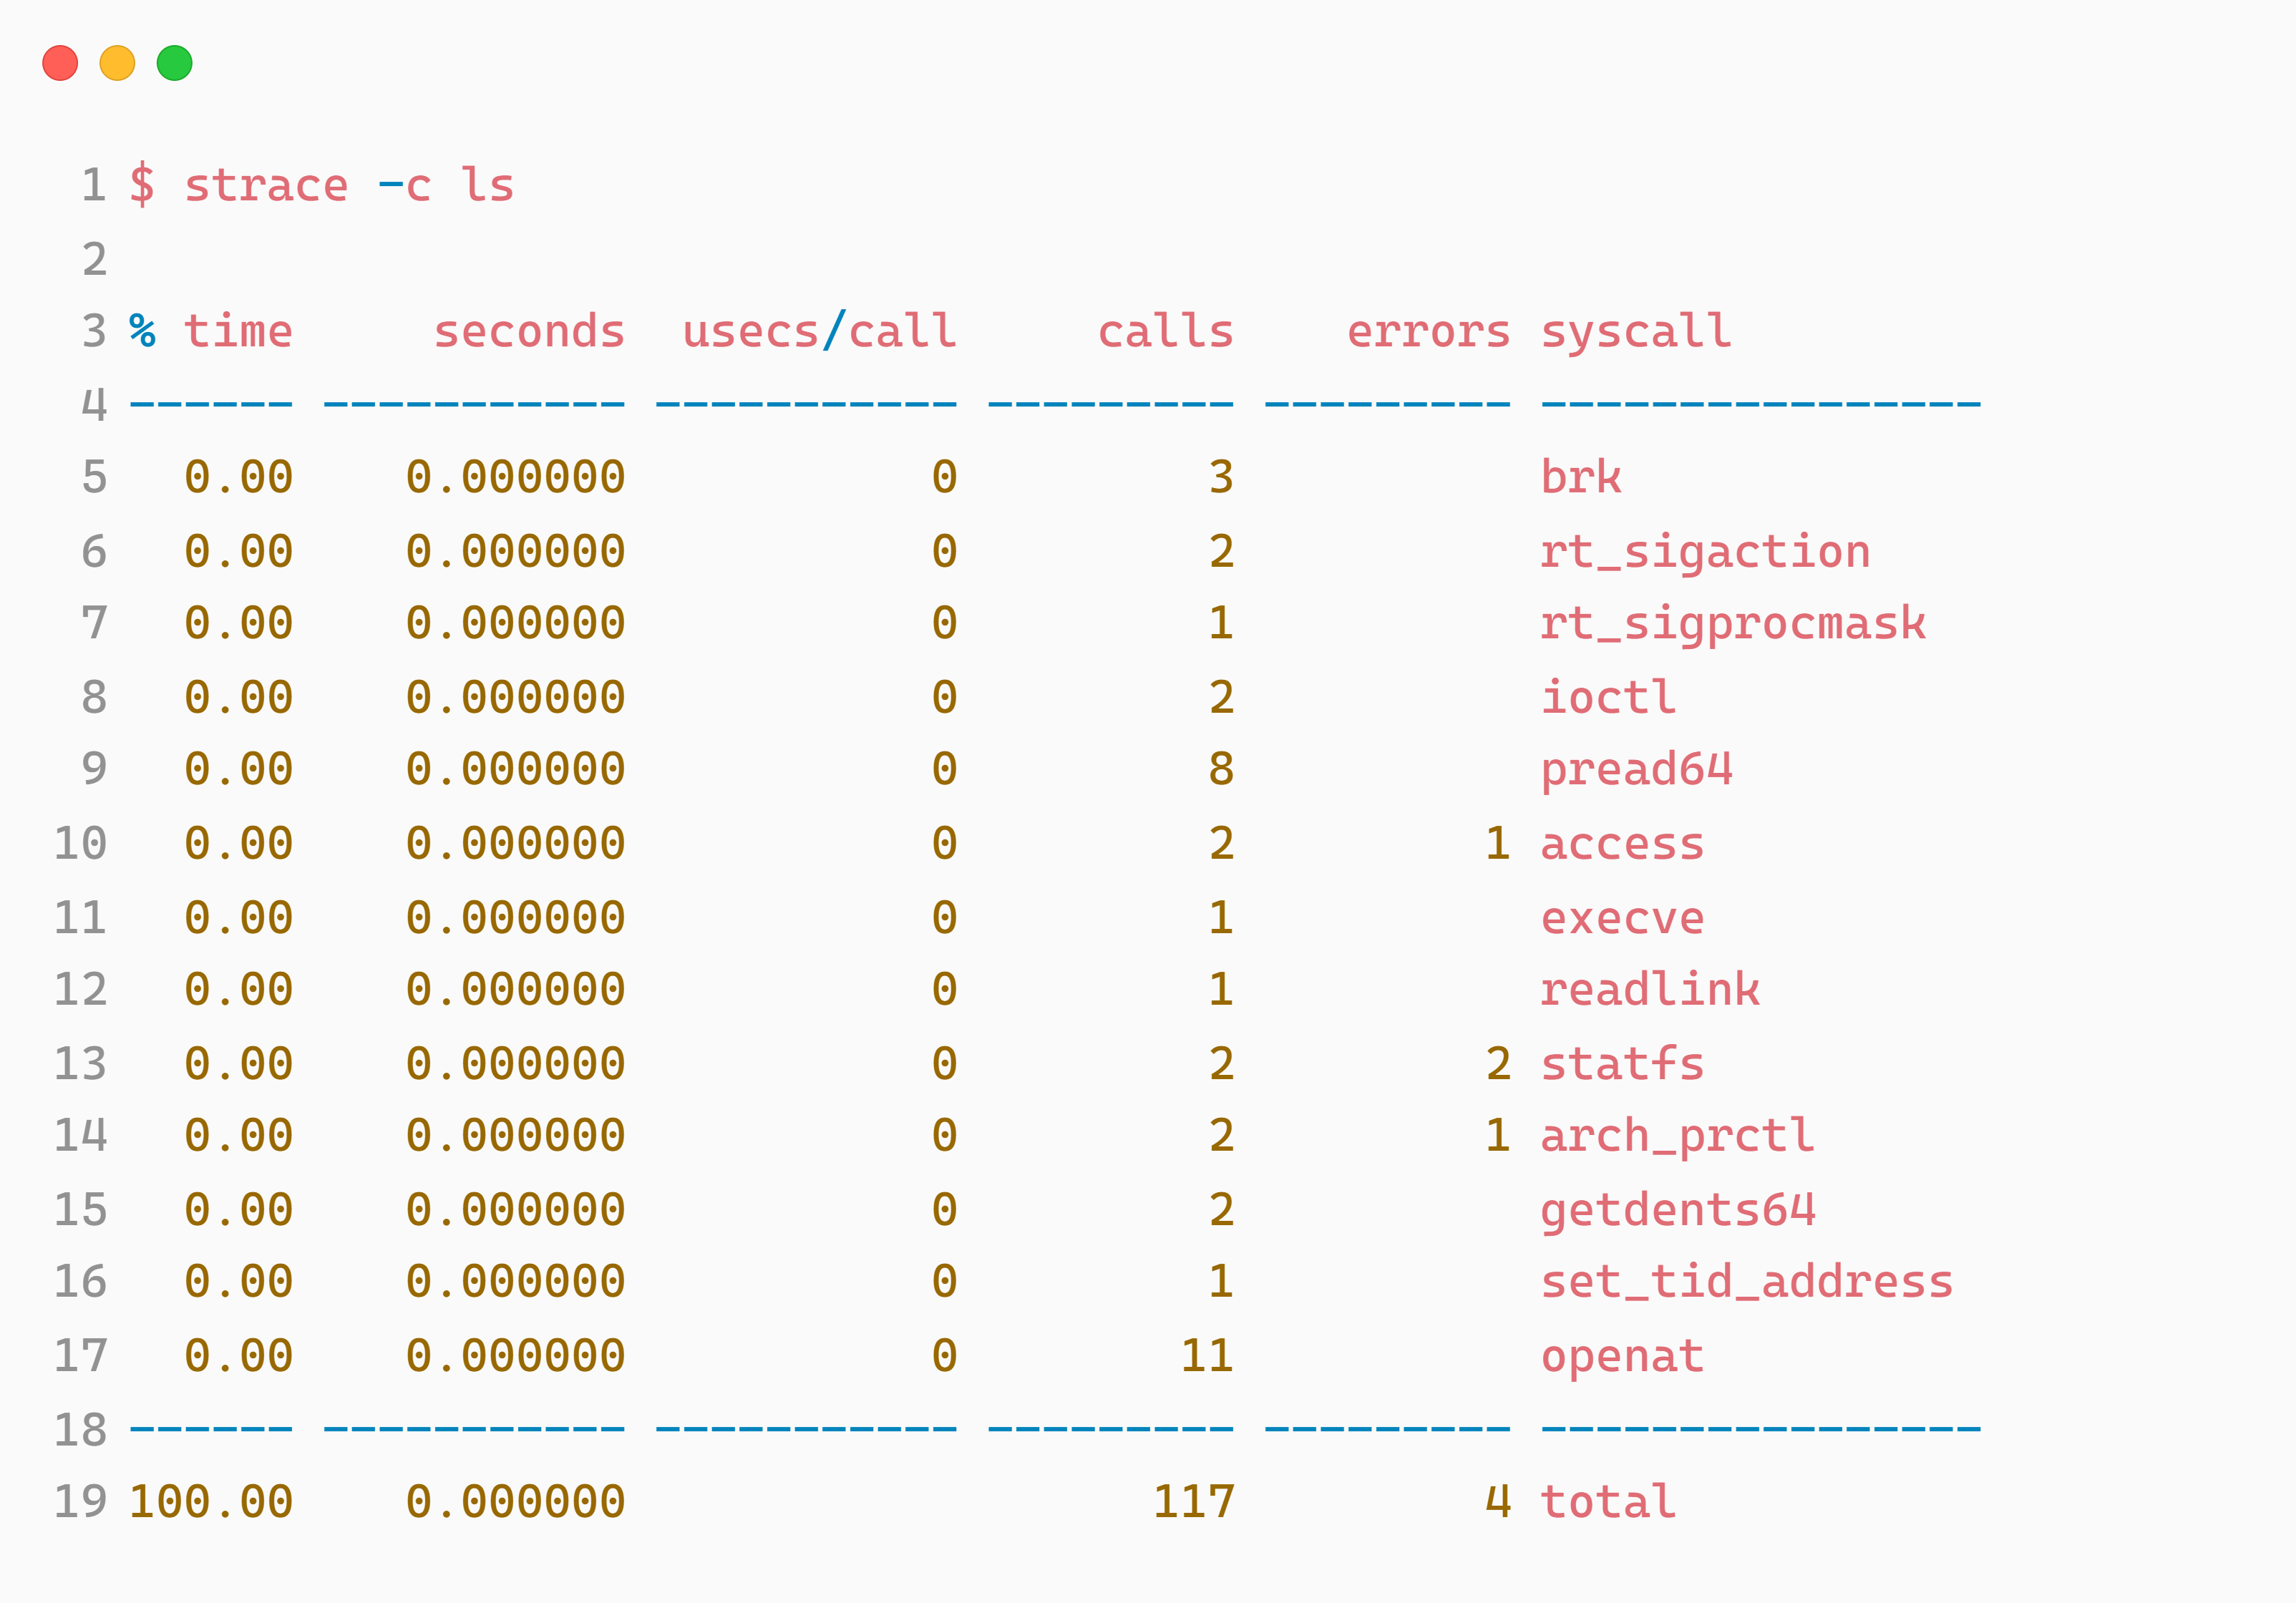
\includegraphics[width=0.80\textwidth]{pic/strace.png}
		\end{itemize}
\end{frame}

\begin{frame}{doxygen}
	\begin{itemize}
		\centering
		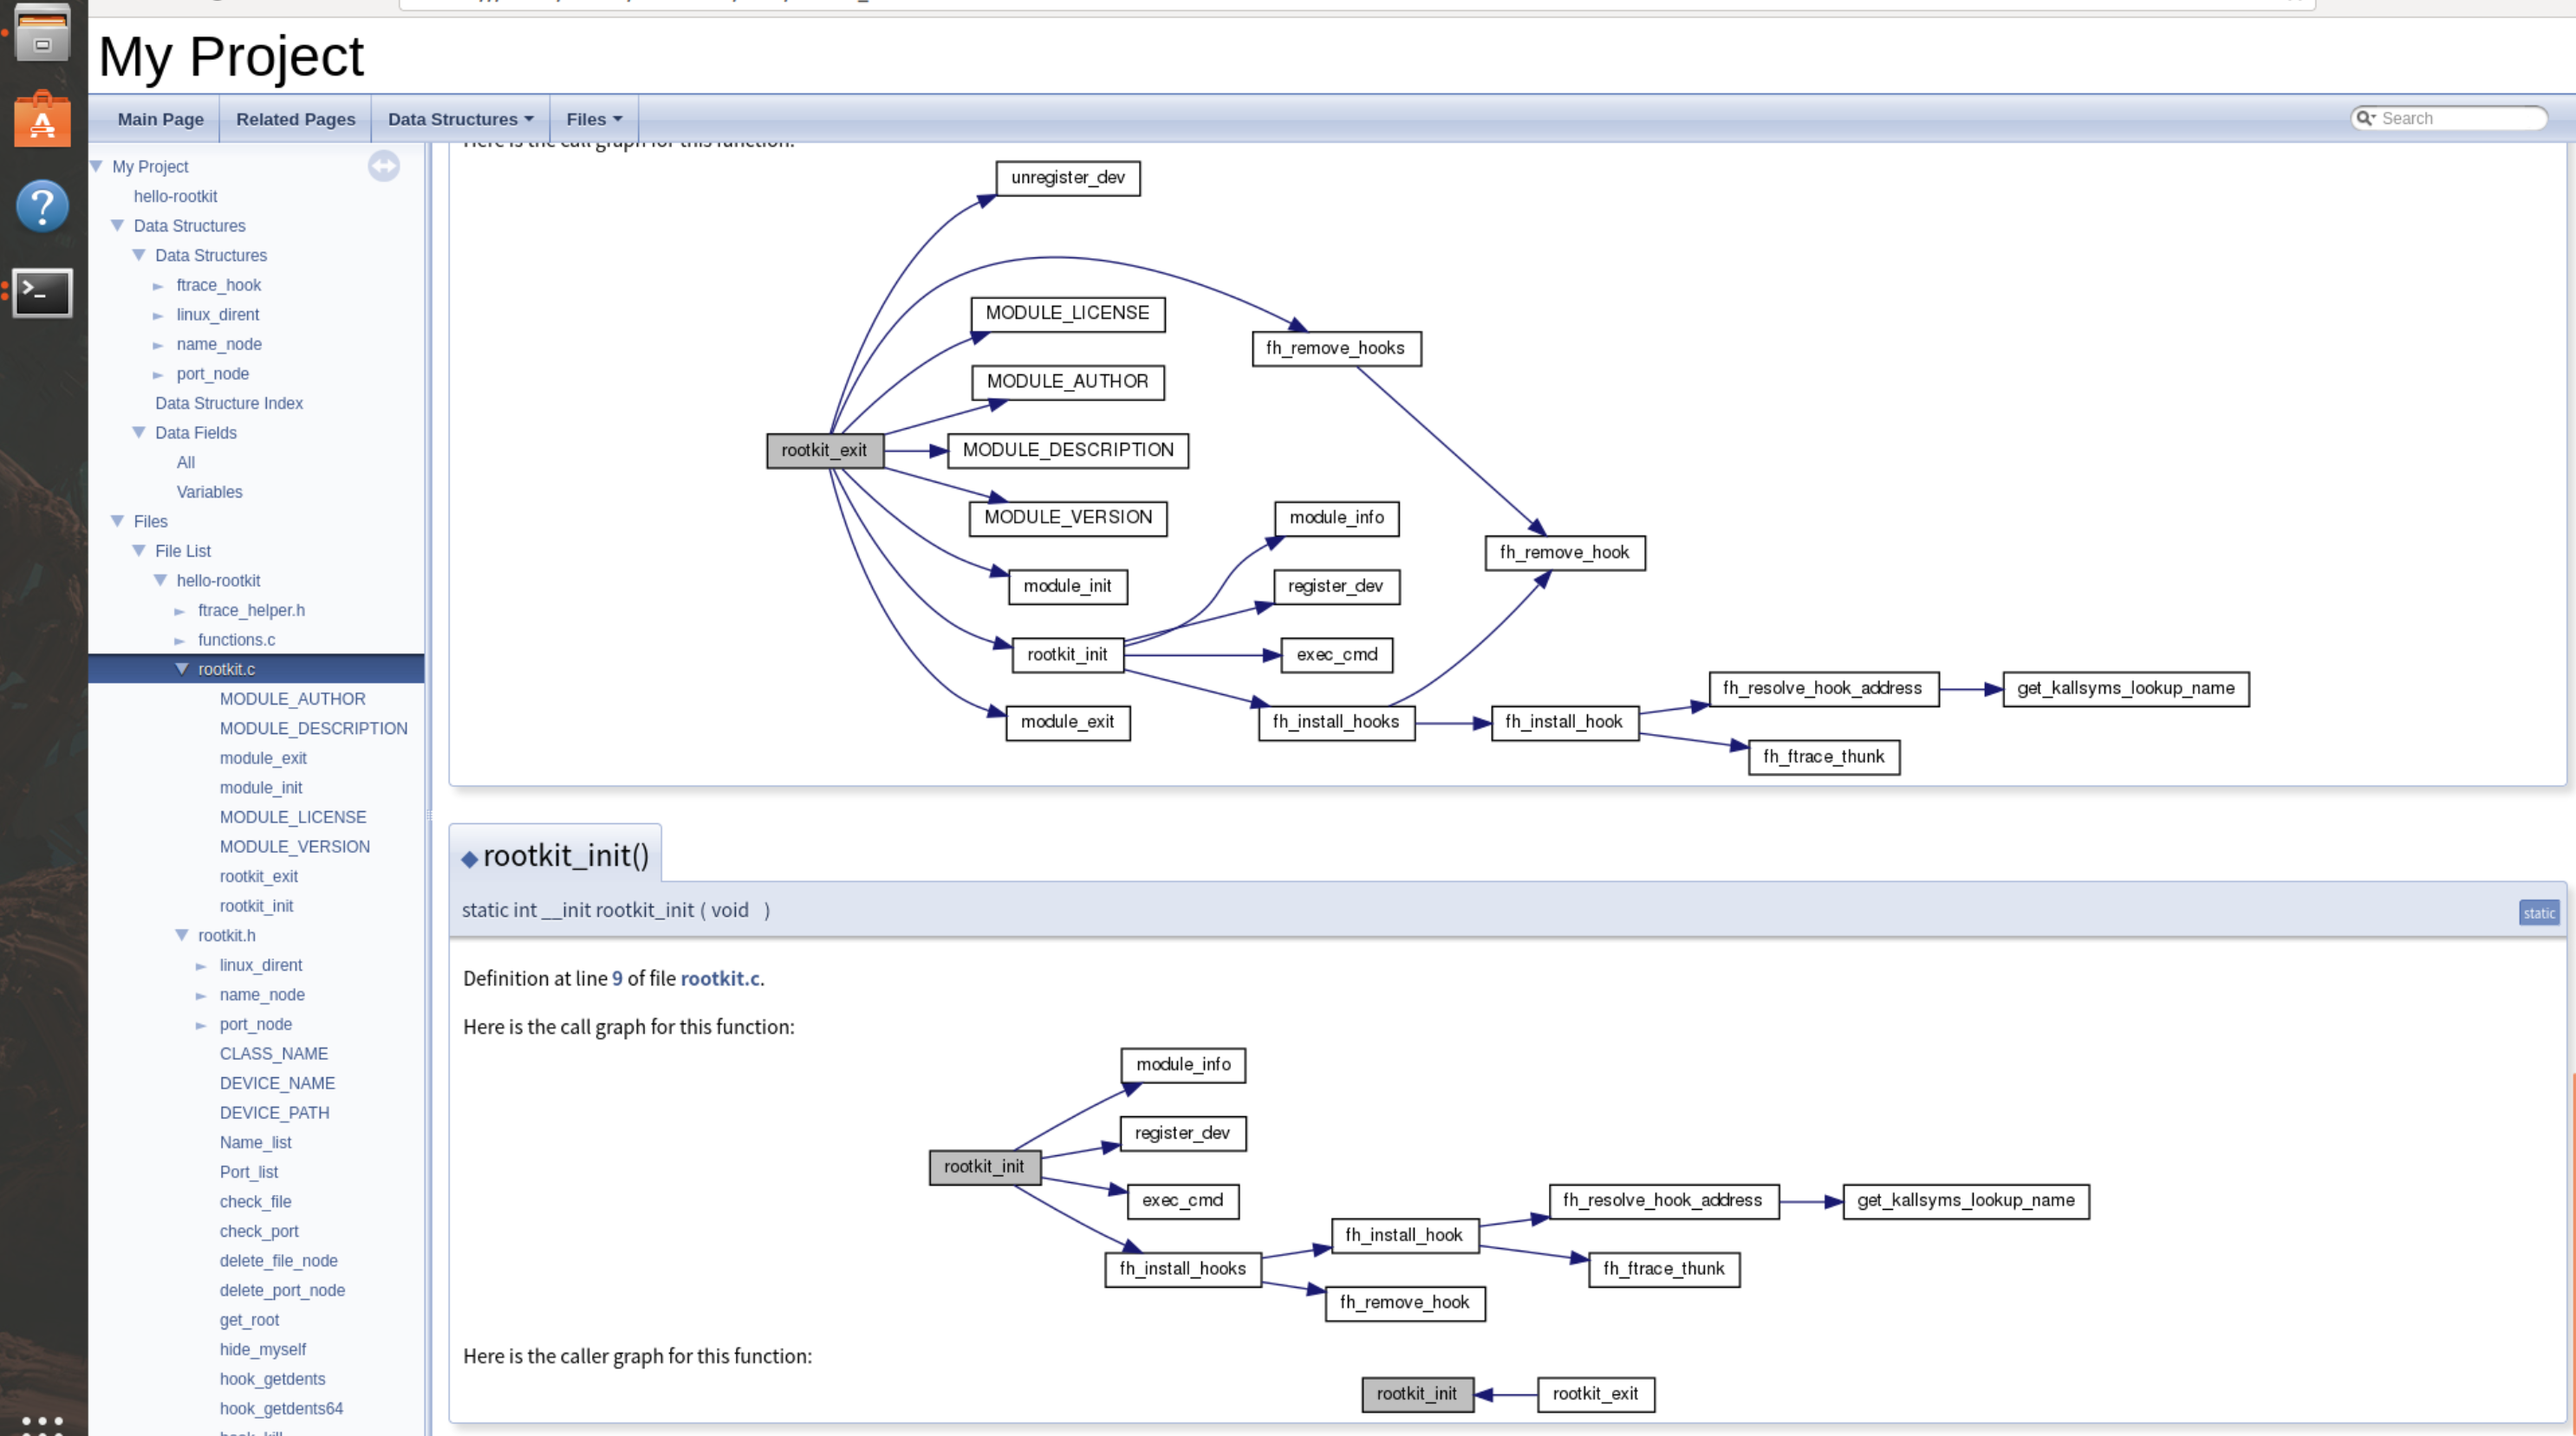
\includegraphics[width=0.95\textwidth]{pic/doxygen.png}
	\end{itemize}
\end{frame}

%====================提权section
\section{提权}

\begin{frame}
    \begin{itemize}
        \item cred是一个记录进程credentials信息的结构体,定义在cred.c头文件中
        \item prepare\_creds()返回当前进程的cred结构
        \item commit\_creds()将这个cred应用于当前进程,因此我们只需要对cred结构体进行修改即可实现提权
    \end{itemize}
	\begin{itemize}
		\centering
		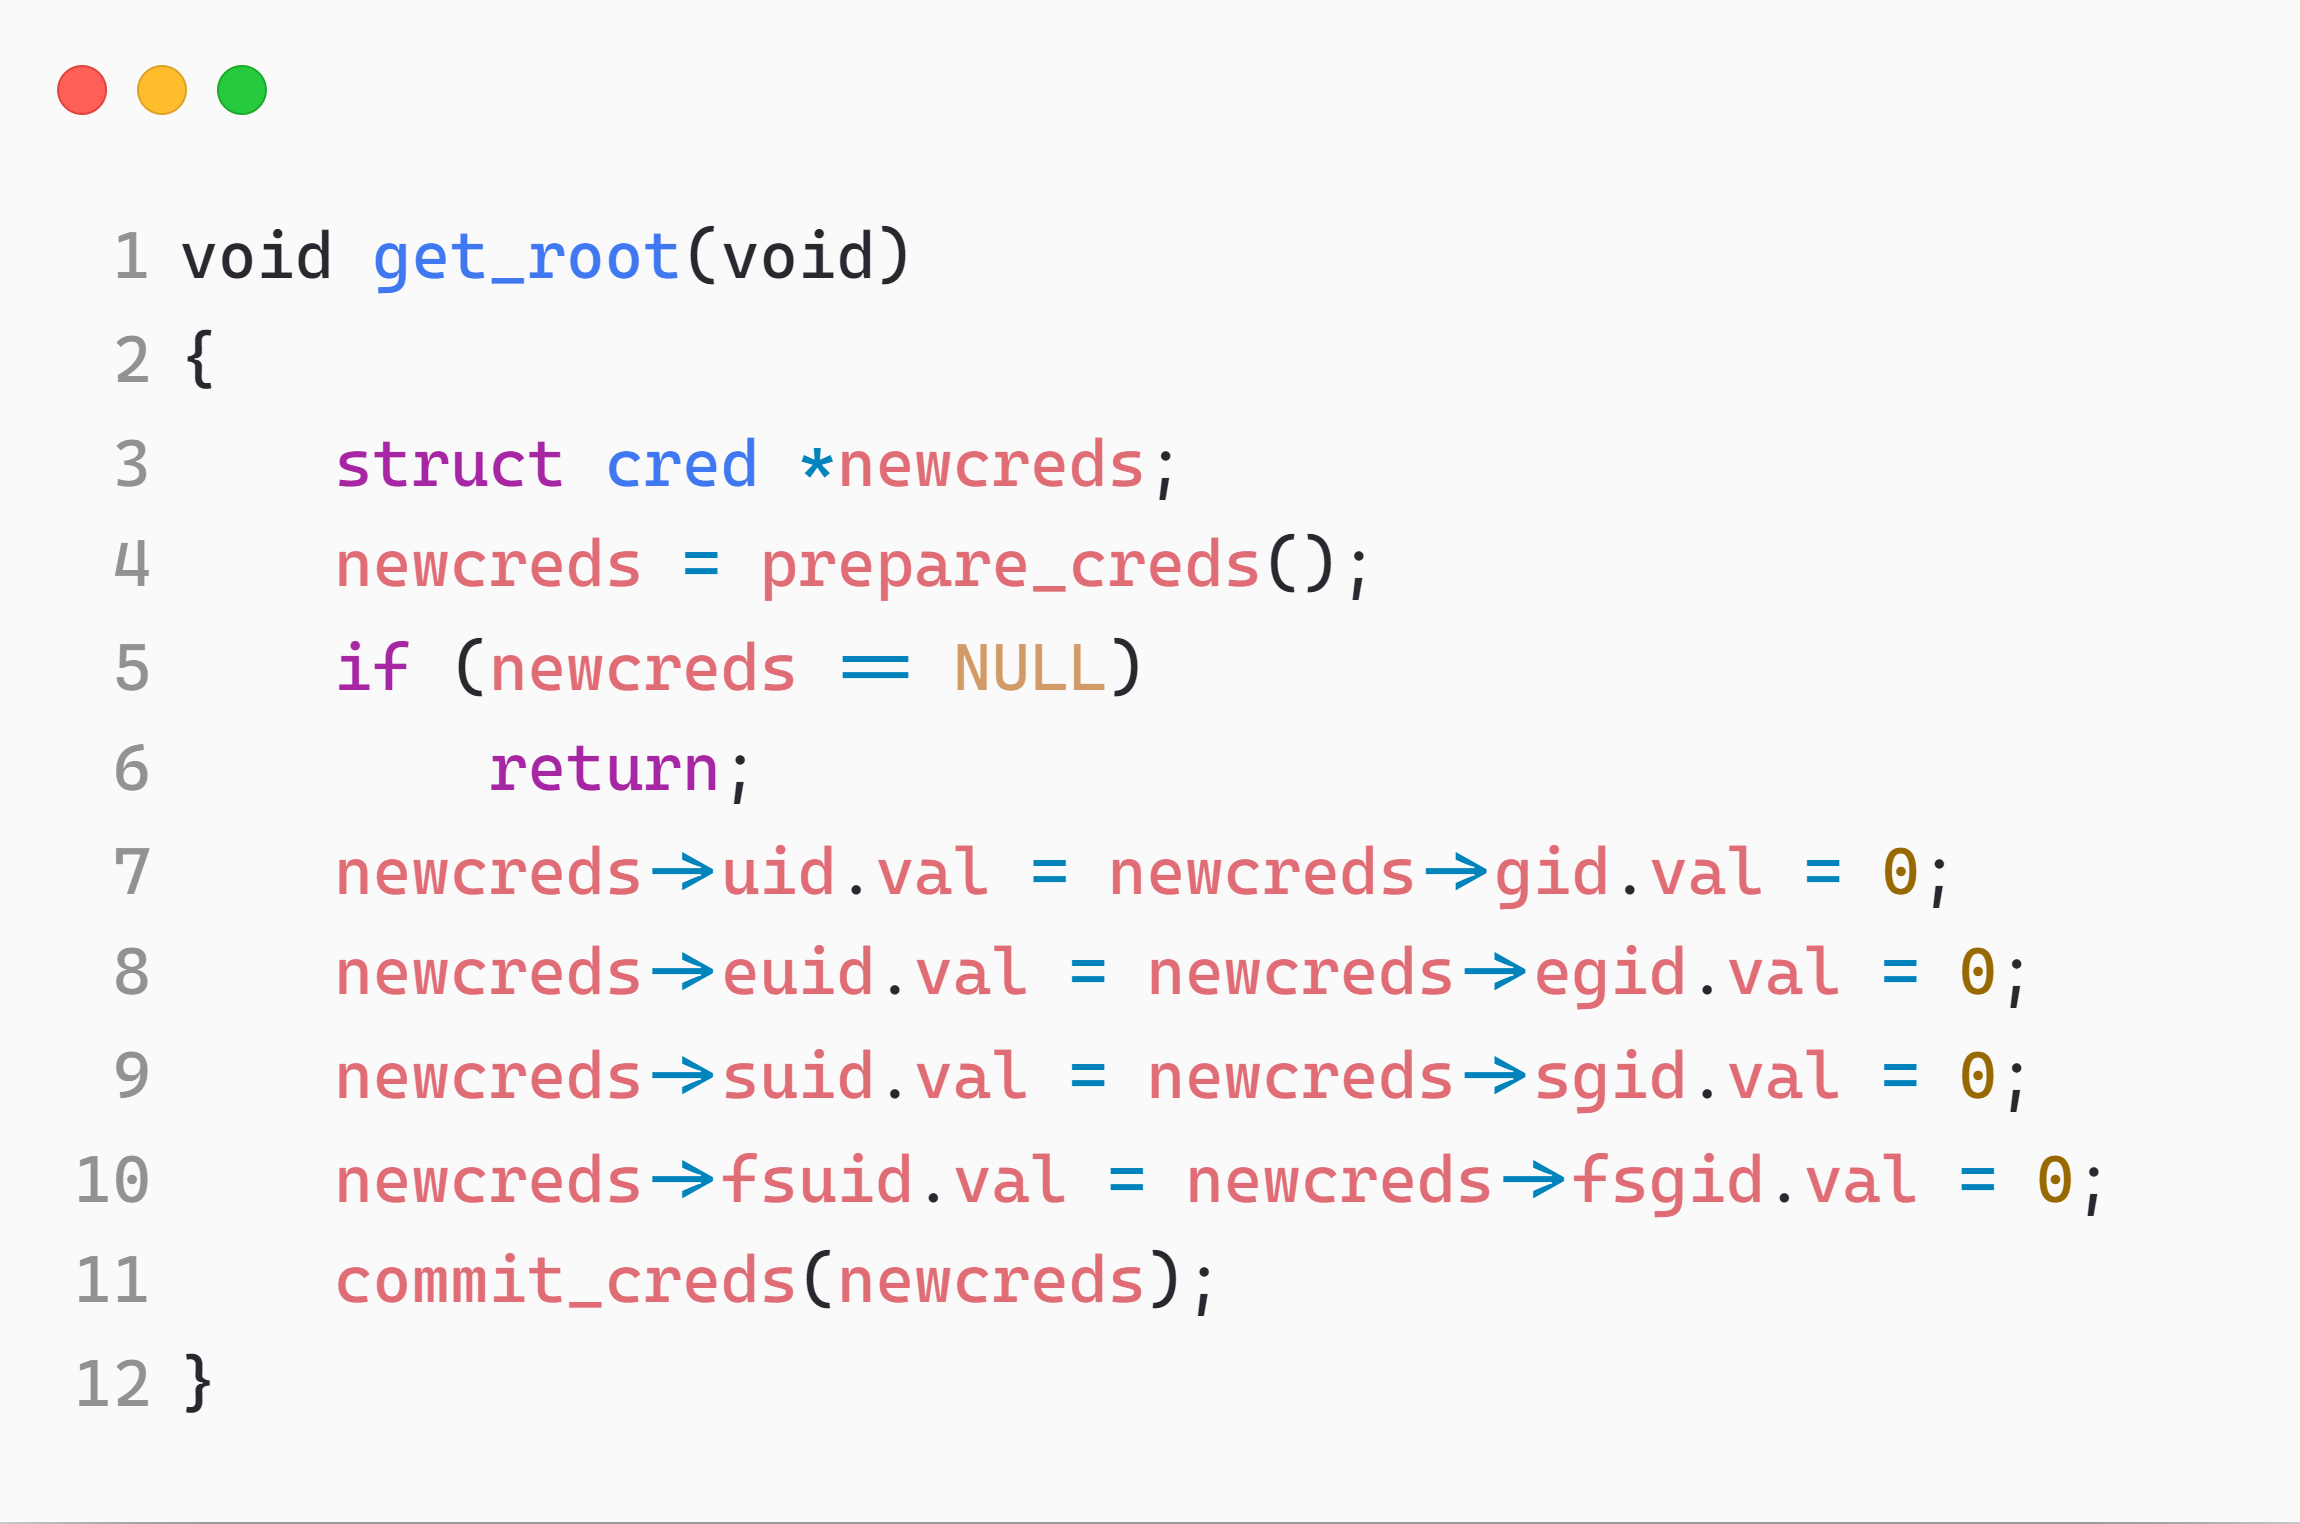
\includegraphics[width=0.80\textwidth]{pic/get-root.png}
	\end{itemize}
\end{frame}

\begin{frame}
	\begin{itemize}
		\item hook kill实现提权
		\item 当我们在shell中输入kill命令的时候会将shell提权到root
		\item 使用id命令验证
	\end{itemize}
	\begin{itemize}
		\centering
		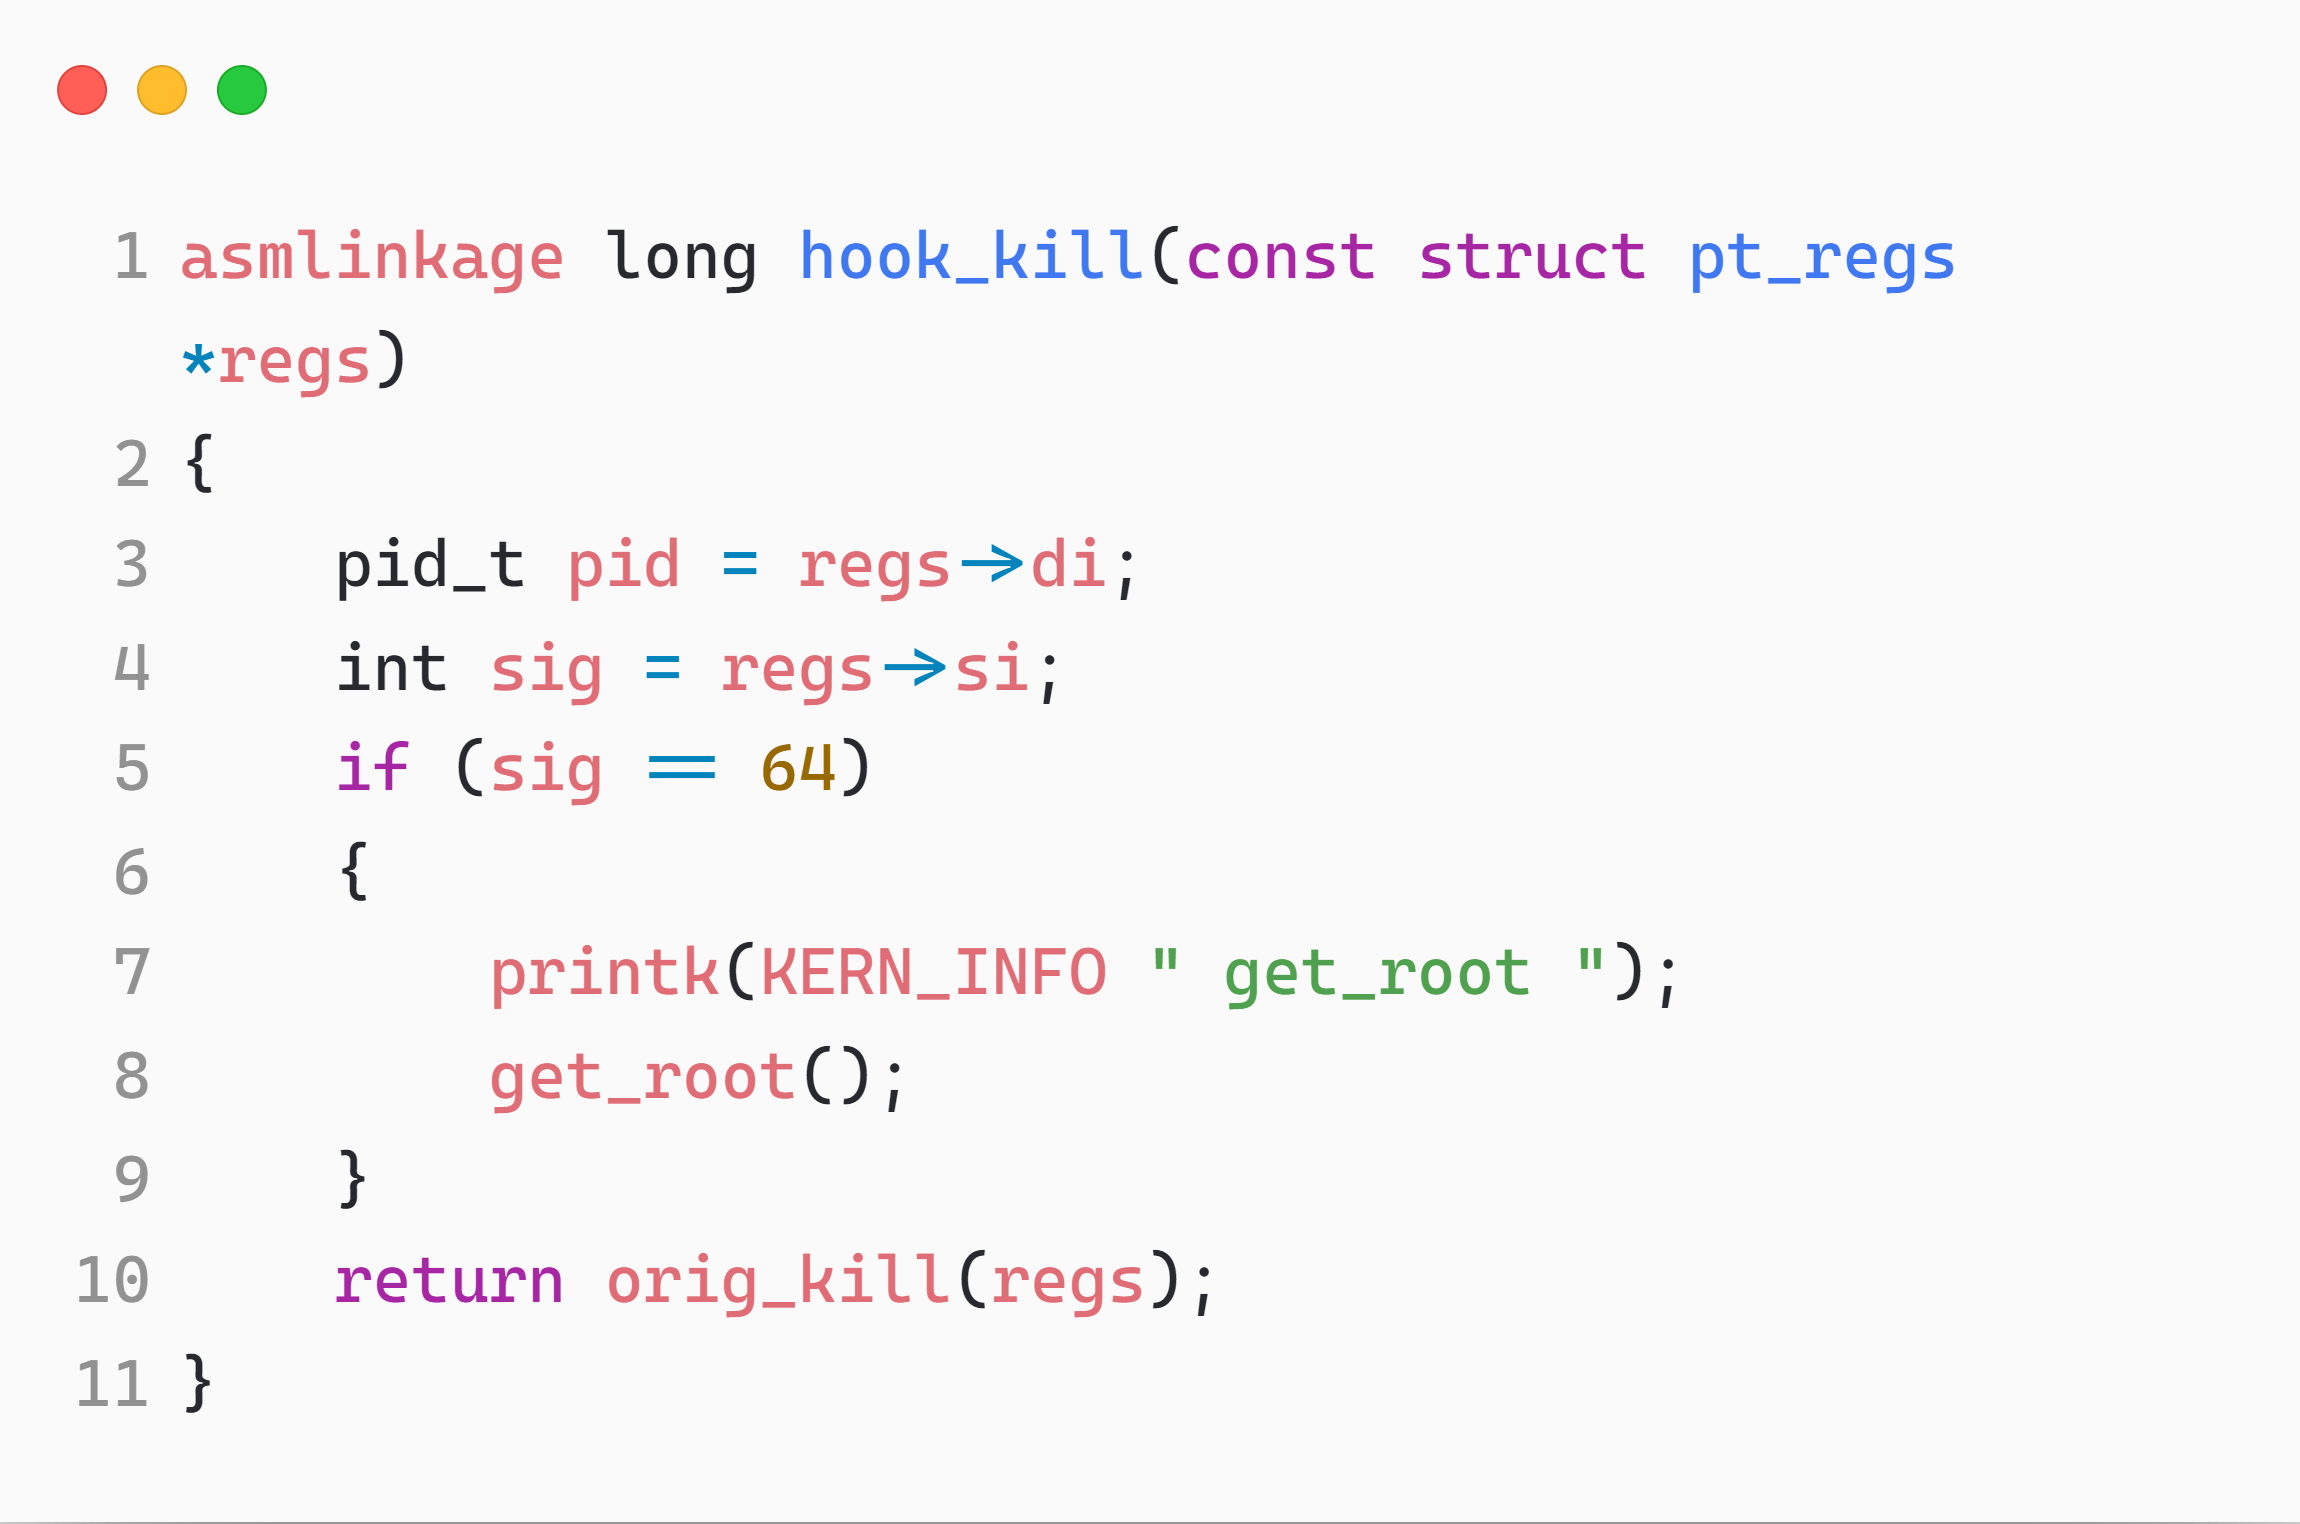
\includegraphics[width=0.80\textwidth]{pic/hookkill.png}
	\end{itemize}
\end{frame}

%====================模块隐藏section
\section{模块隐藏}

\begin{frame}
	\begin{itemize}
		\item 内核使用module结构体存储模块信息
		\item module结构体封装了list双向链表,下面的源码来自module.h
		\item 把rootkit模块的list从全局链表中删除即可
		\item THIS\_MODULE宏指向当前模块的module struct
	\end{itemize}

\end{frame}

\begin{frame}
\begin{itemize}
	\centering
	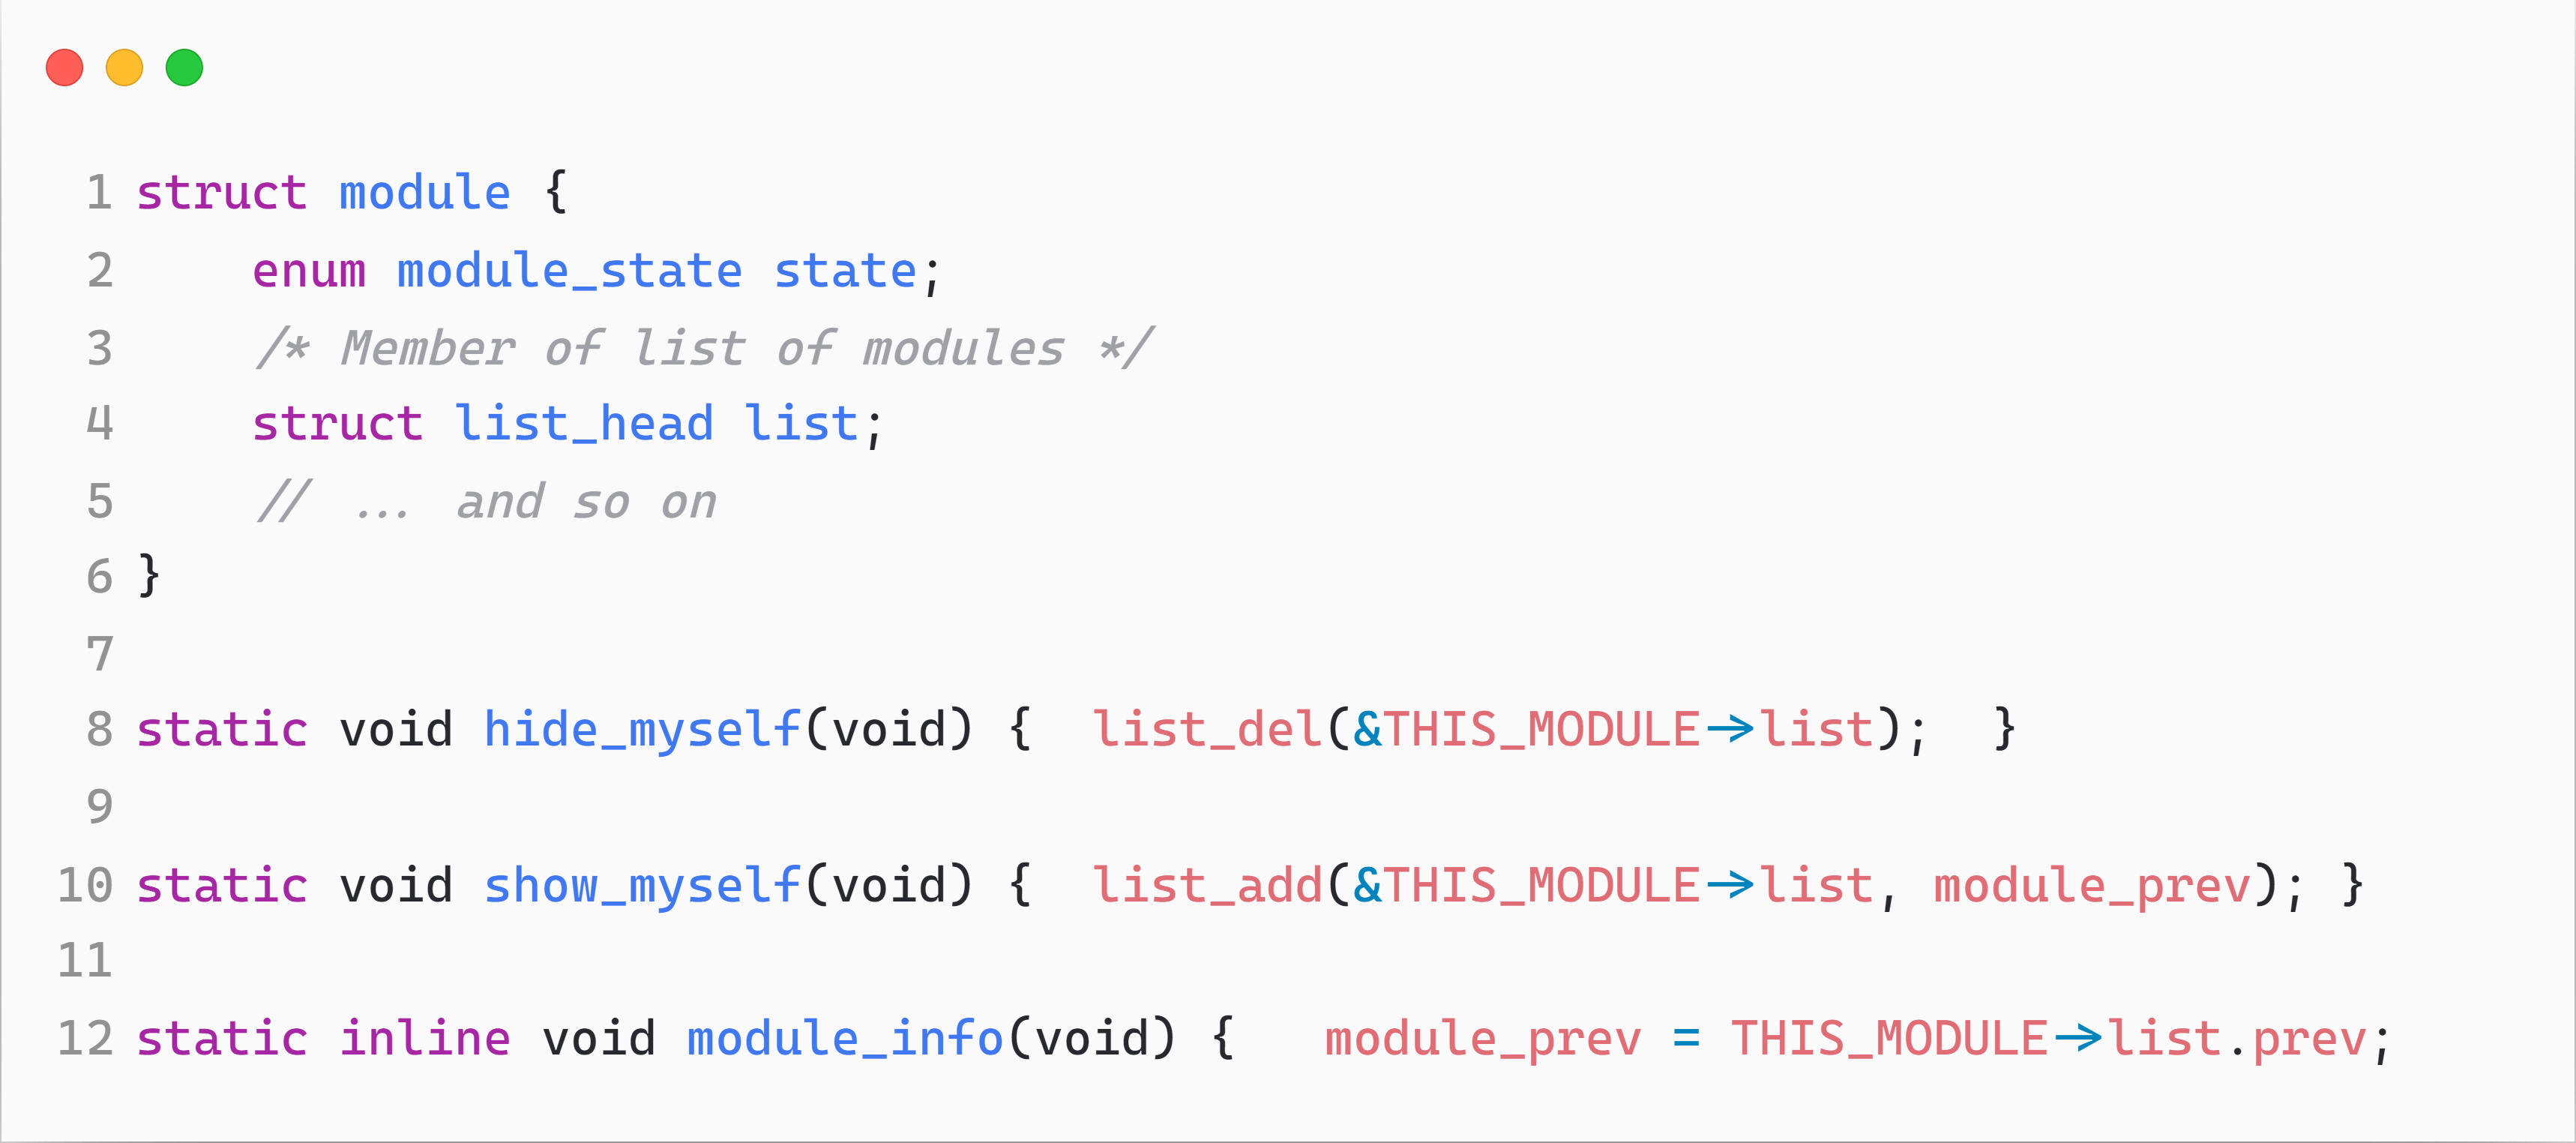
\includegraphics[width=0.95\textwidth]{pic/module.png}
\end{itemize}
\end{frame}

%====================文件隐藏section
\section{文件隐藏}

\begin{frame}
	\begin{itemize}
		\item getdents64函数获取目录的entry并返回读取字节数
		\item hook getdents64函数从而达到隐藏文件的目的
		\item 某些内核版本使用getdents函数,64是为了处理更大的文件系统和偏移而设计的
	\end{itemize}
	\begin{itemize}
		\centering
		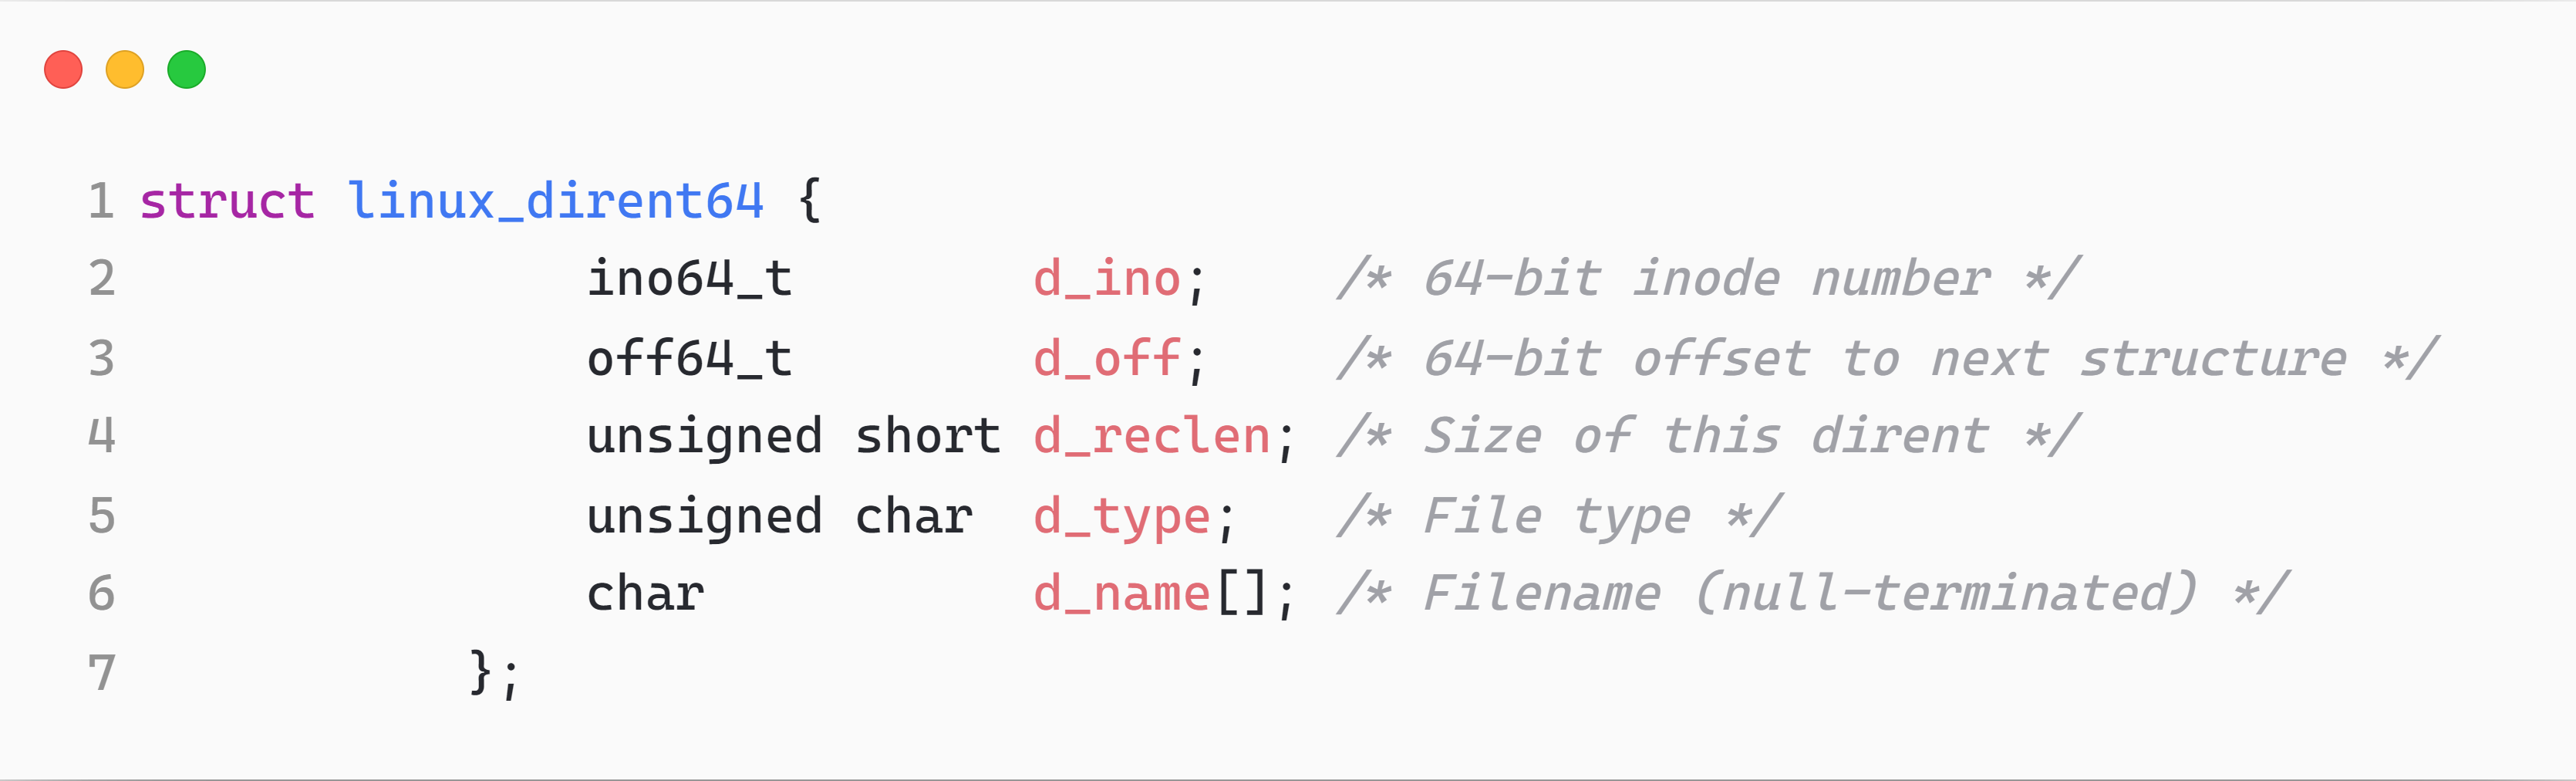
\includegraphics[width=0.90\textwidth]{pic/dirent64.png}
	\end{itemize}
\end{frame}

\begin{frame}
	\begin{itemize}
		\item 文件隐藏函数的实现,省略了一些细节
		\item hook getdents与getdents64有一些不同
	\end{itemize}
	\begin{itemize}
		\centering
		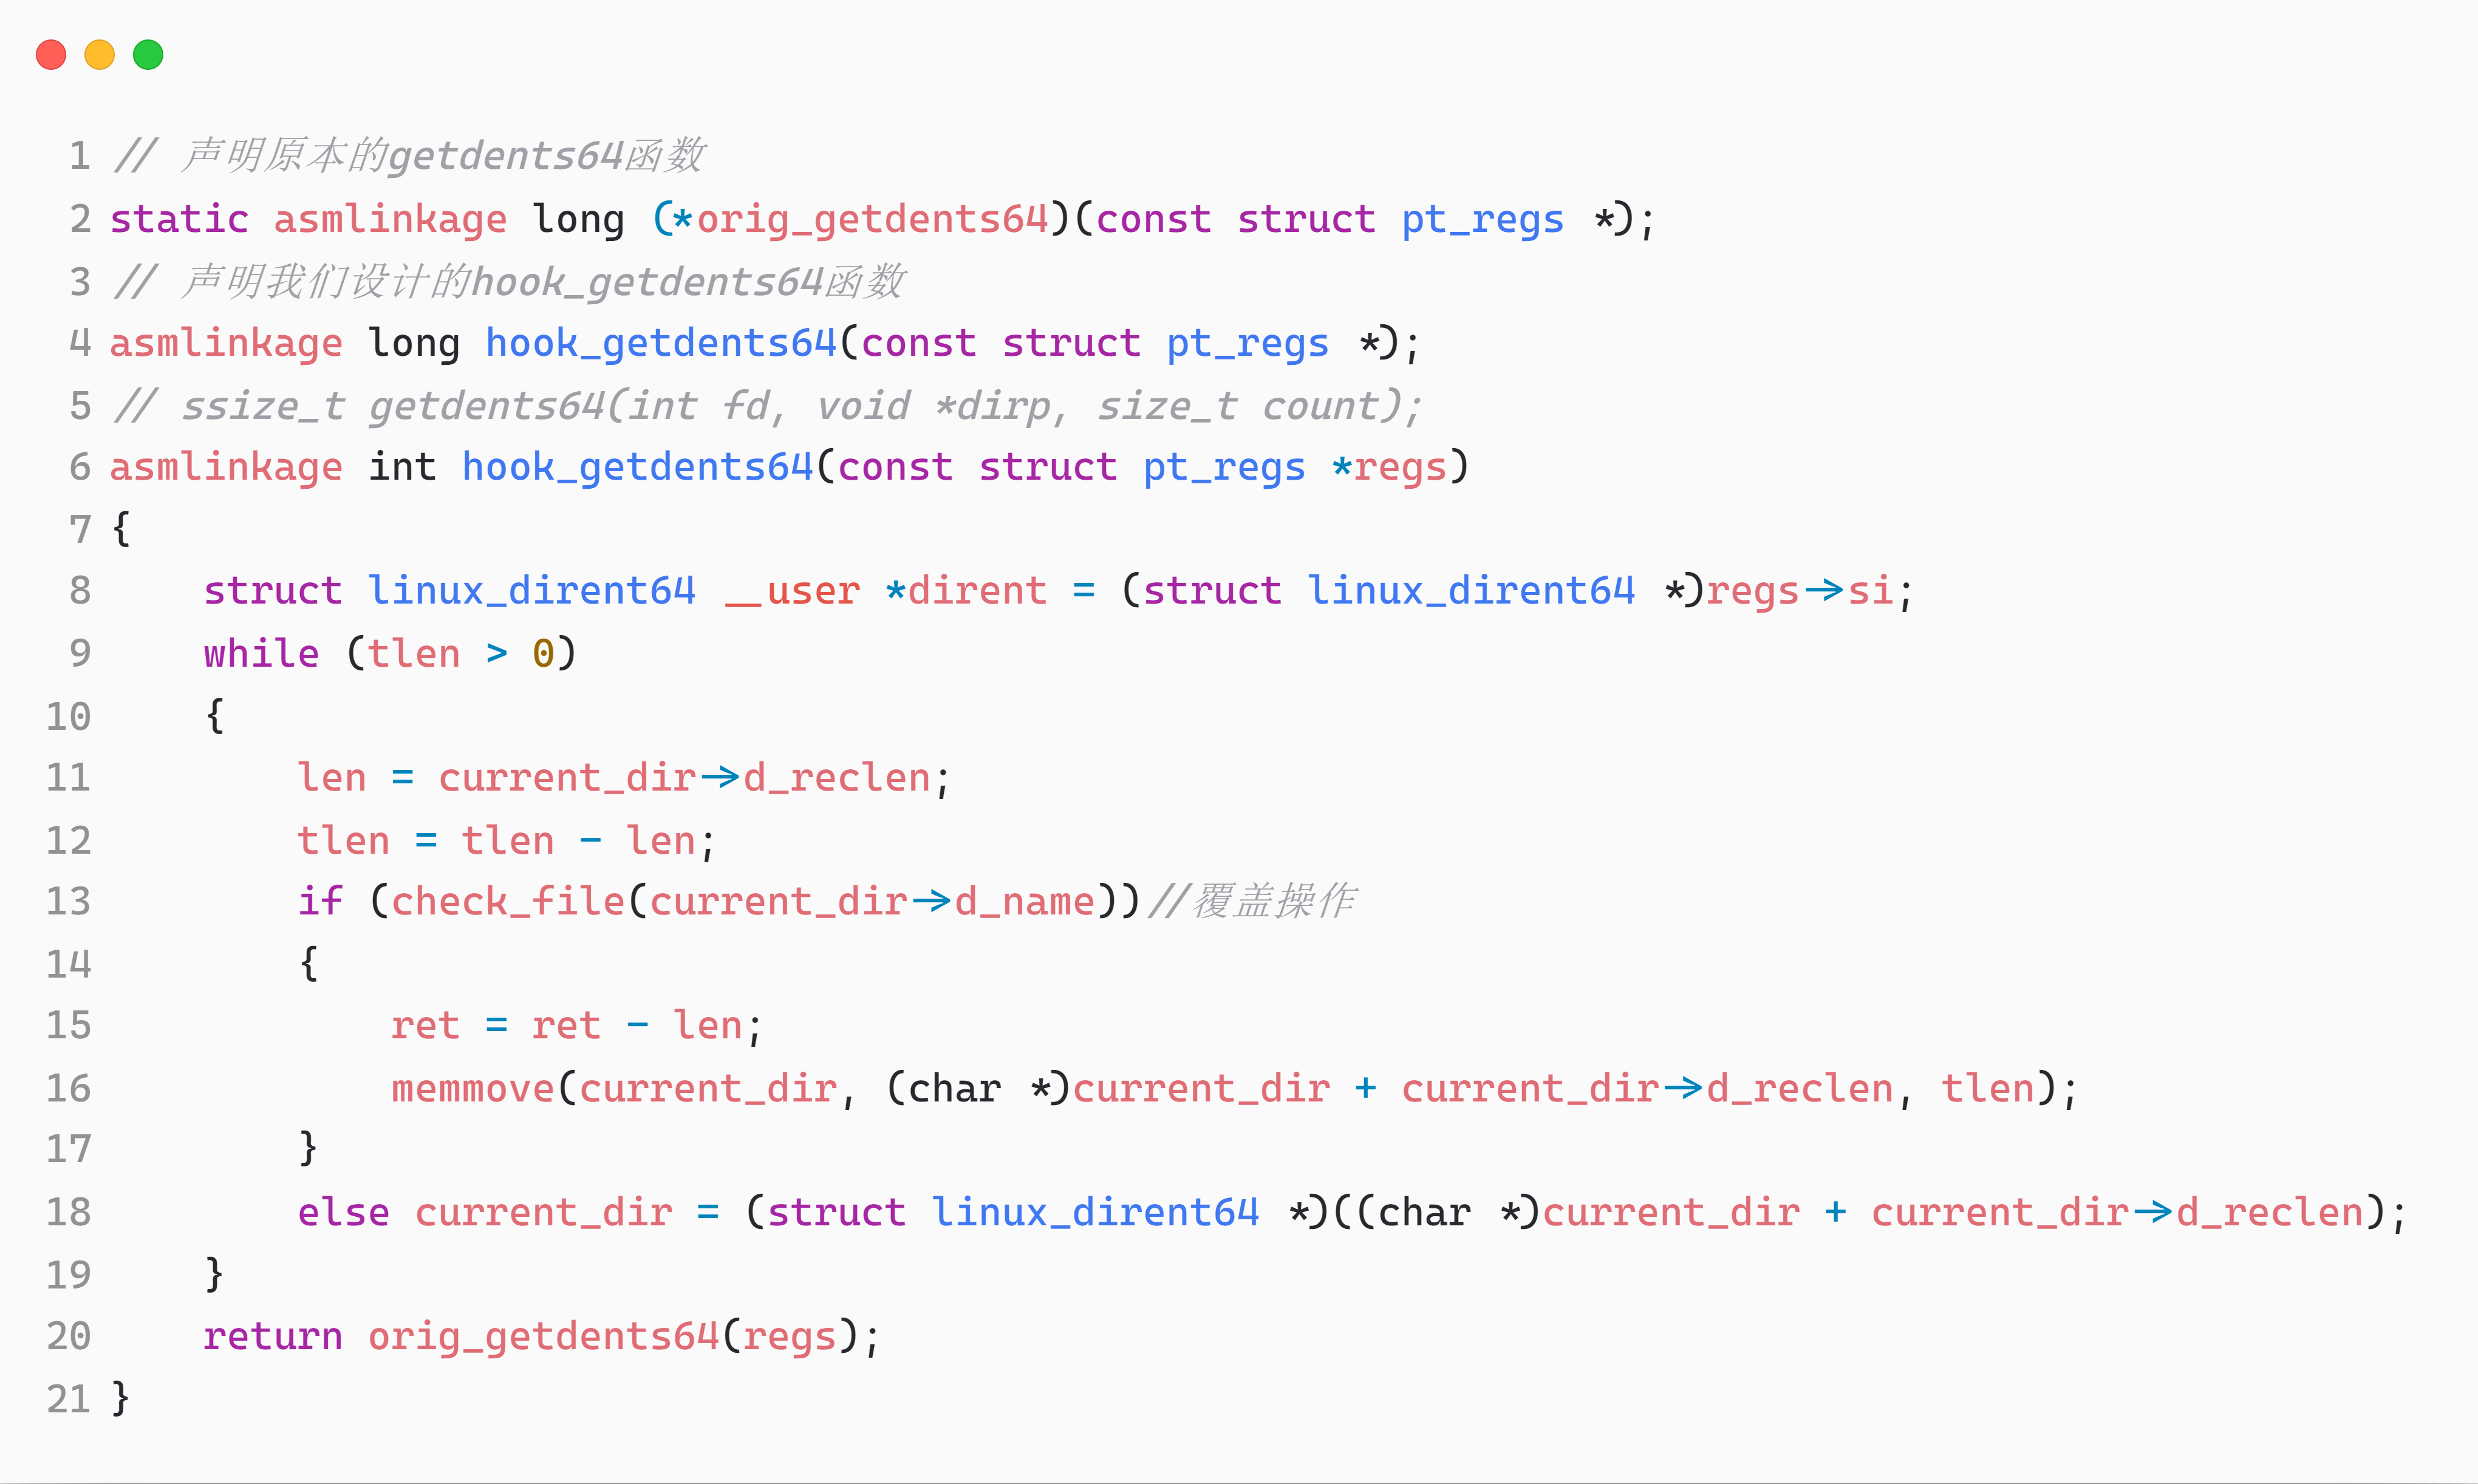
\includegraphics[width=0.90\textwidth]{pic/hook_getdents64.png}
	\end{itemize}
\end{frame}

%====================进程隐藏section
\section{进程隐藏}
\begin{frame}
	\begin{itemize}
		\item linux内核维护了task\_struct和pid两个链表,分布记录了进程的task\_struct结构和pid结构
		\item 将rootkit相关的task\_struct和pid都摘除列表
		\item 实现思路
		\begin{itemize}
			\item 根据pid用find\_vpid()找到对应的pid结构体
			\item 用pid\_task()找到对应的task struct
			\item hlist\_del\_rcu对task\_struct 结点进行脱链,并用INIT\_HLIST\_NODE设置task\_struct 的前后指针
			\item 根据task\_struct 找到对应的pid 的结点,利用hlist\_del\_rcu进行脱链
			\item 将隐藏的进程加到hide\_list\_header 链表
			\item 恢复进程时,通过list\_for\_each\_entry\_safe来遍历hide\_list\_header链表
		\end{itemize}
	\end{itemize}
\end{frame}

\begin{frame}
	\begin{itemize}
		\centering
		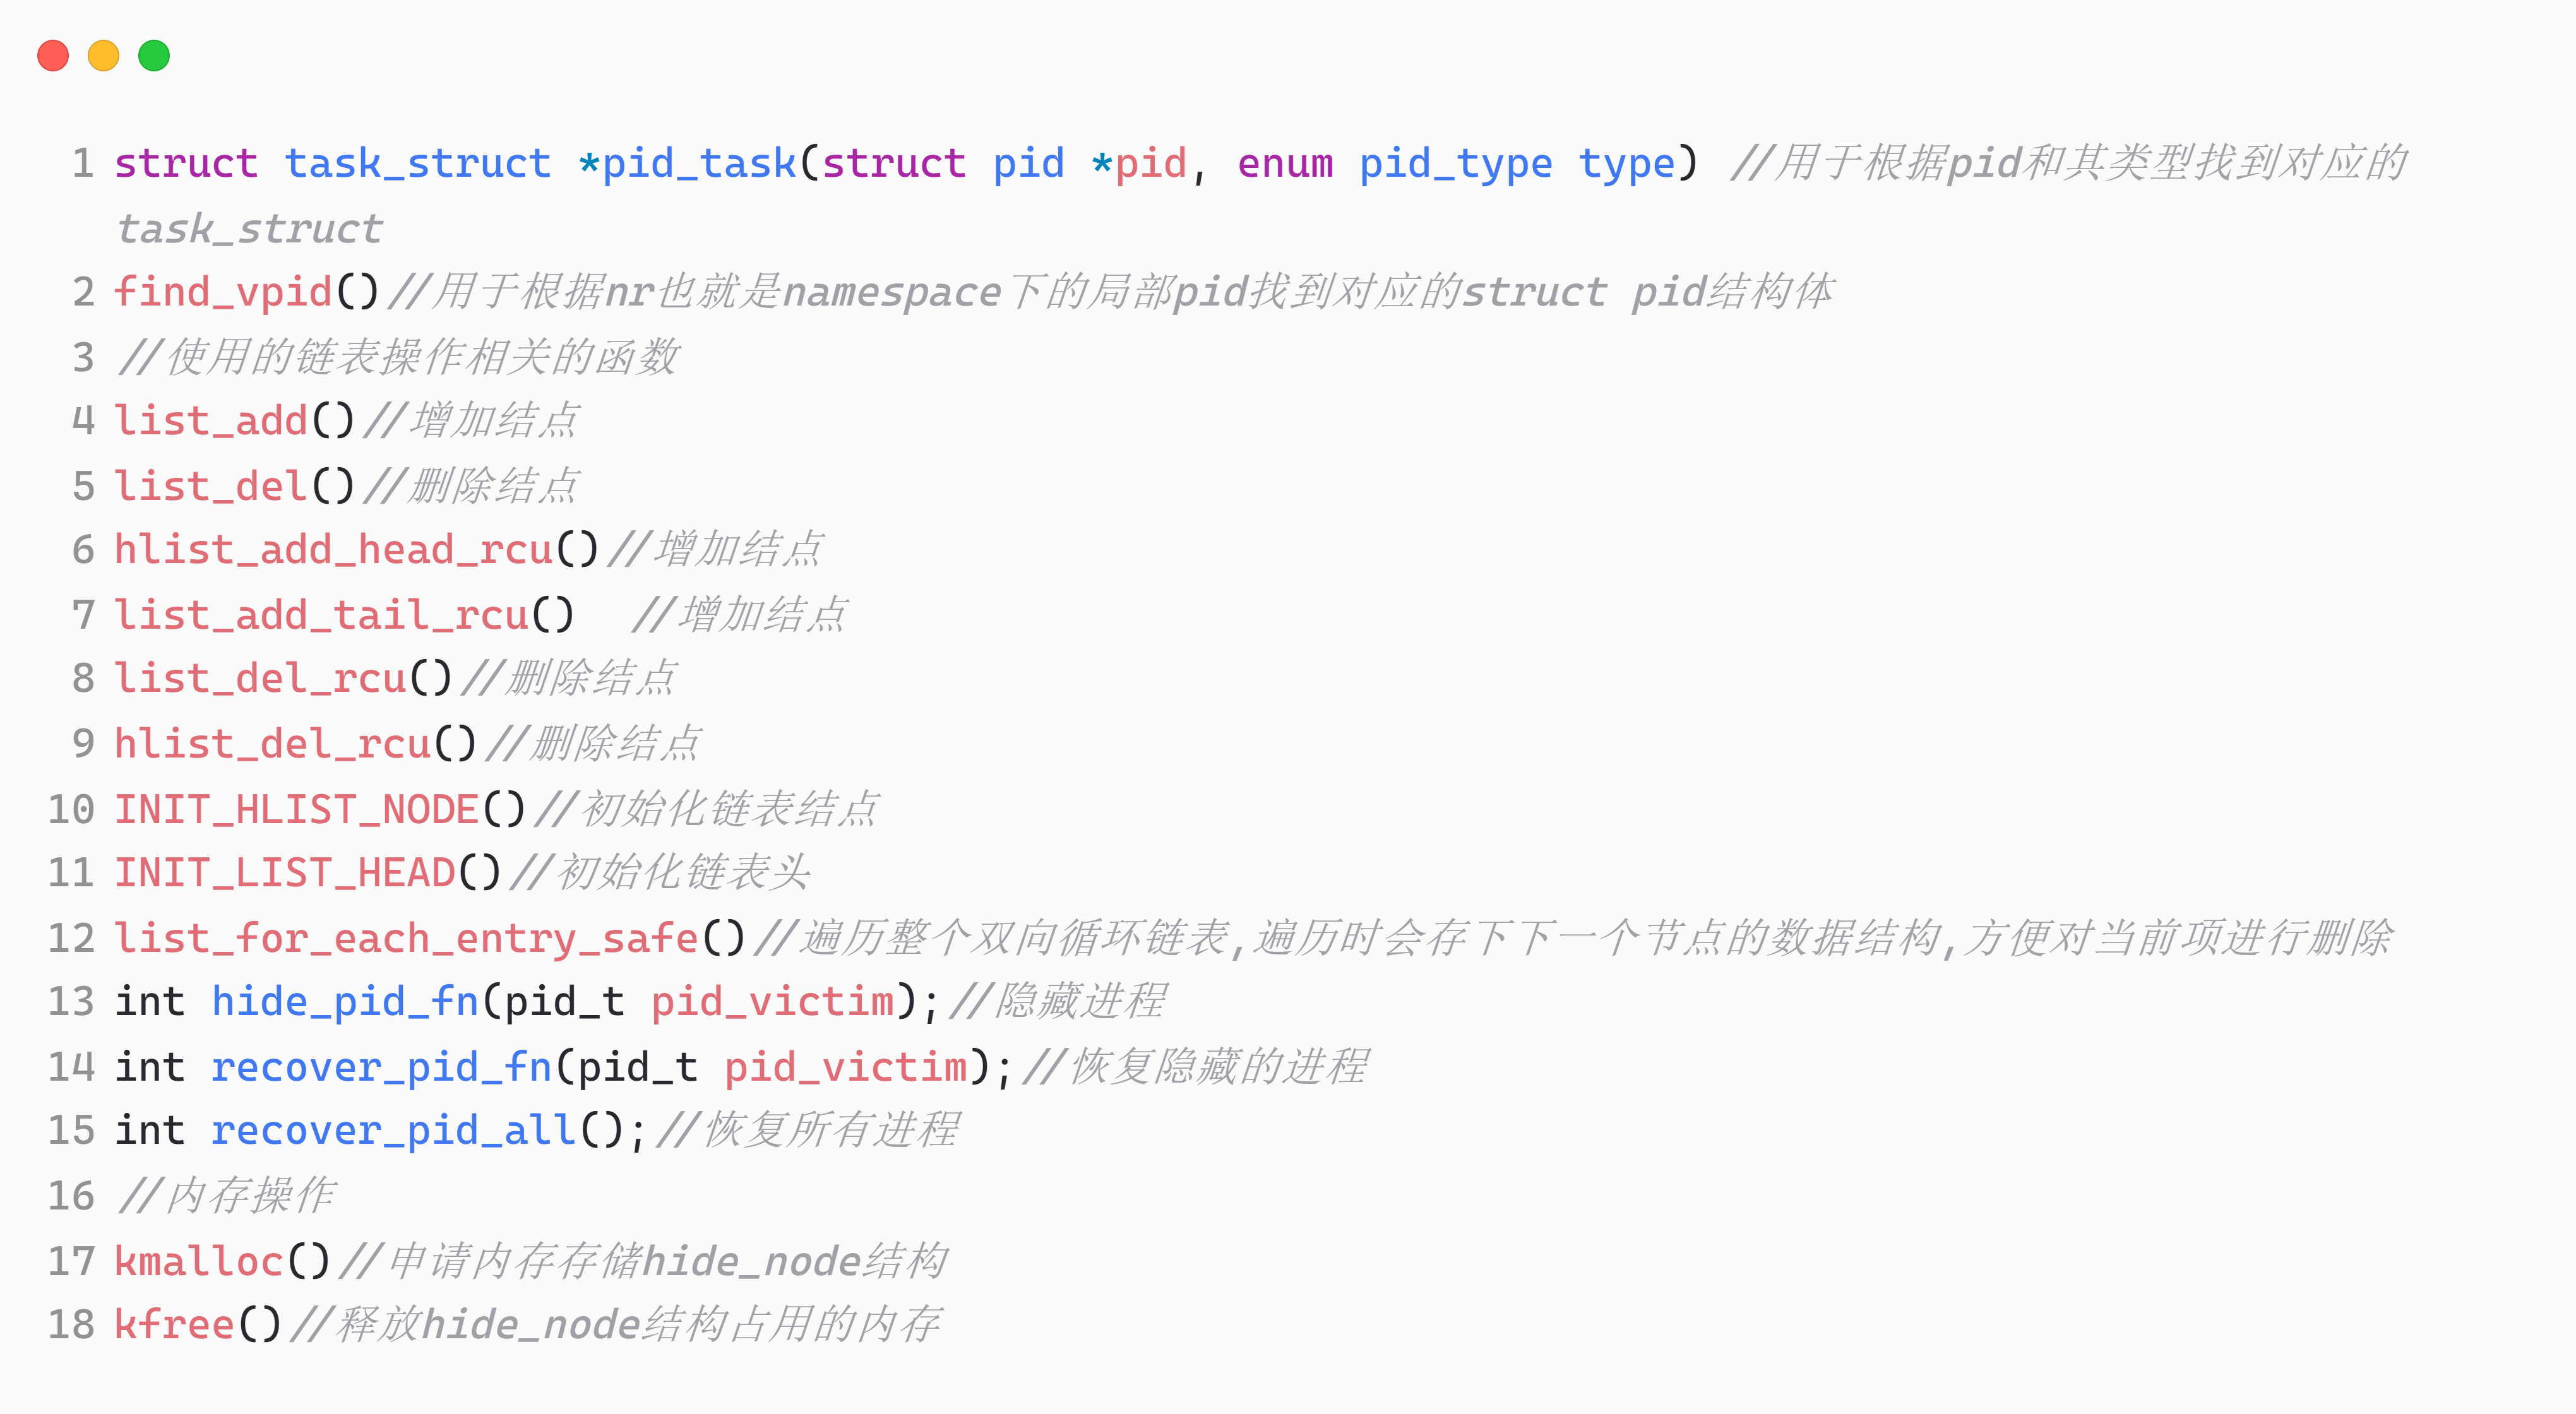
\includegraphics[width=0.95\textwidth]{pic/pid.png}
	\end{itemize}
\end{frame}


%====================端口隐藏section
\section{端口隐藏}
\begin{frame}
	\begin{itemize}
		\item netstat在读取端口信息时会读取以下四个序列文件/proc/net/tcp、/proc/net/udp、/proc/net/tcp6/、/proc/net/udp6
		\item show函数是netstat要输出的信息
		\item 对应的数据结构如下
	\end{itemize}
	\begin{itemize}
		\centering
		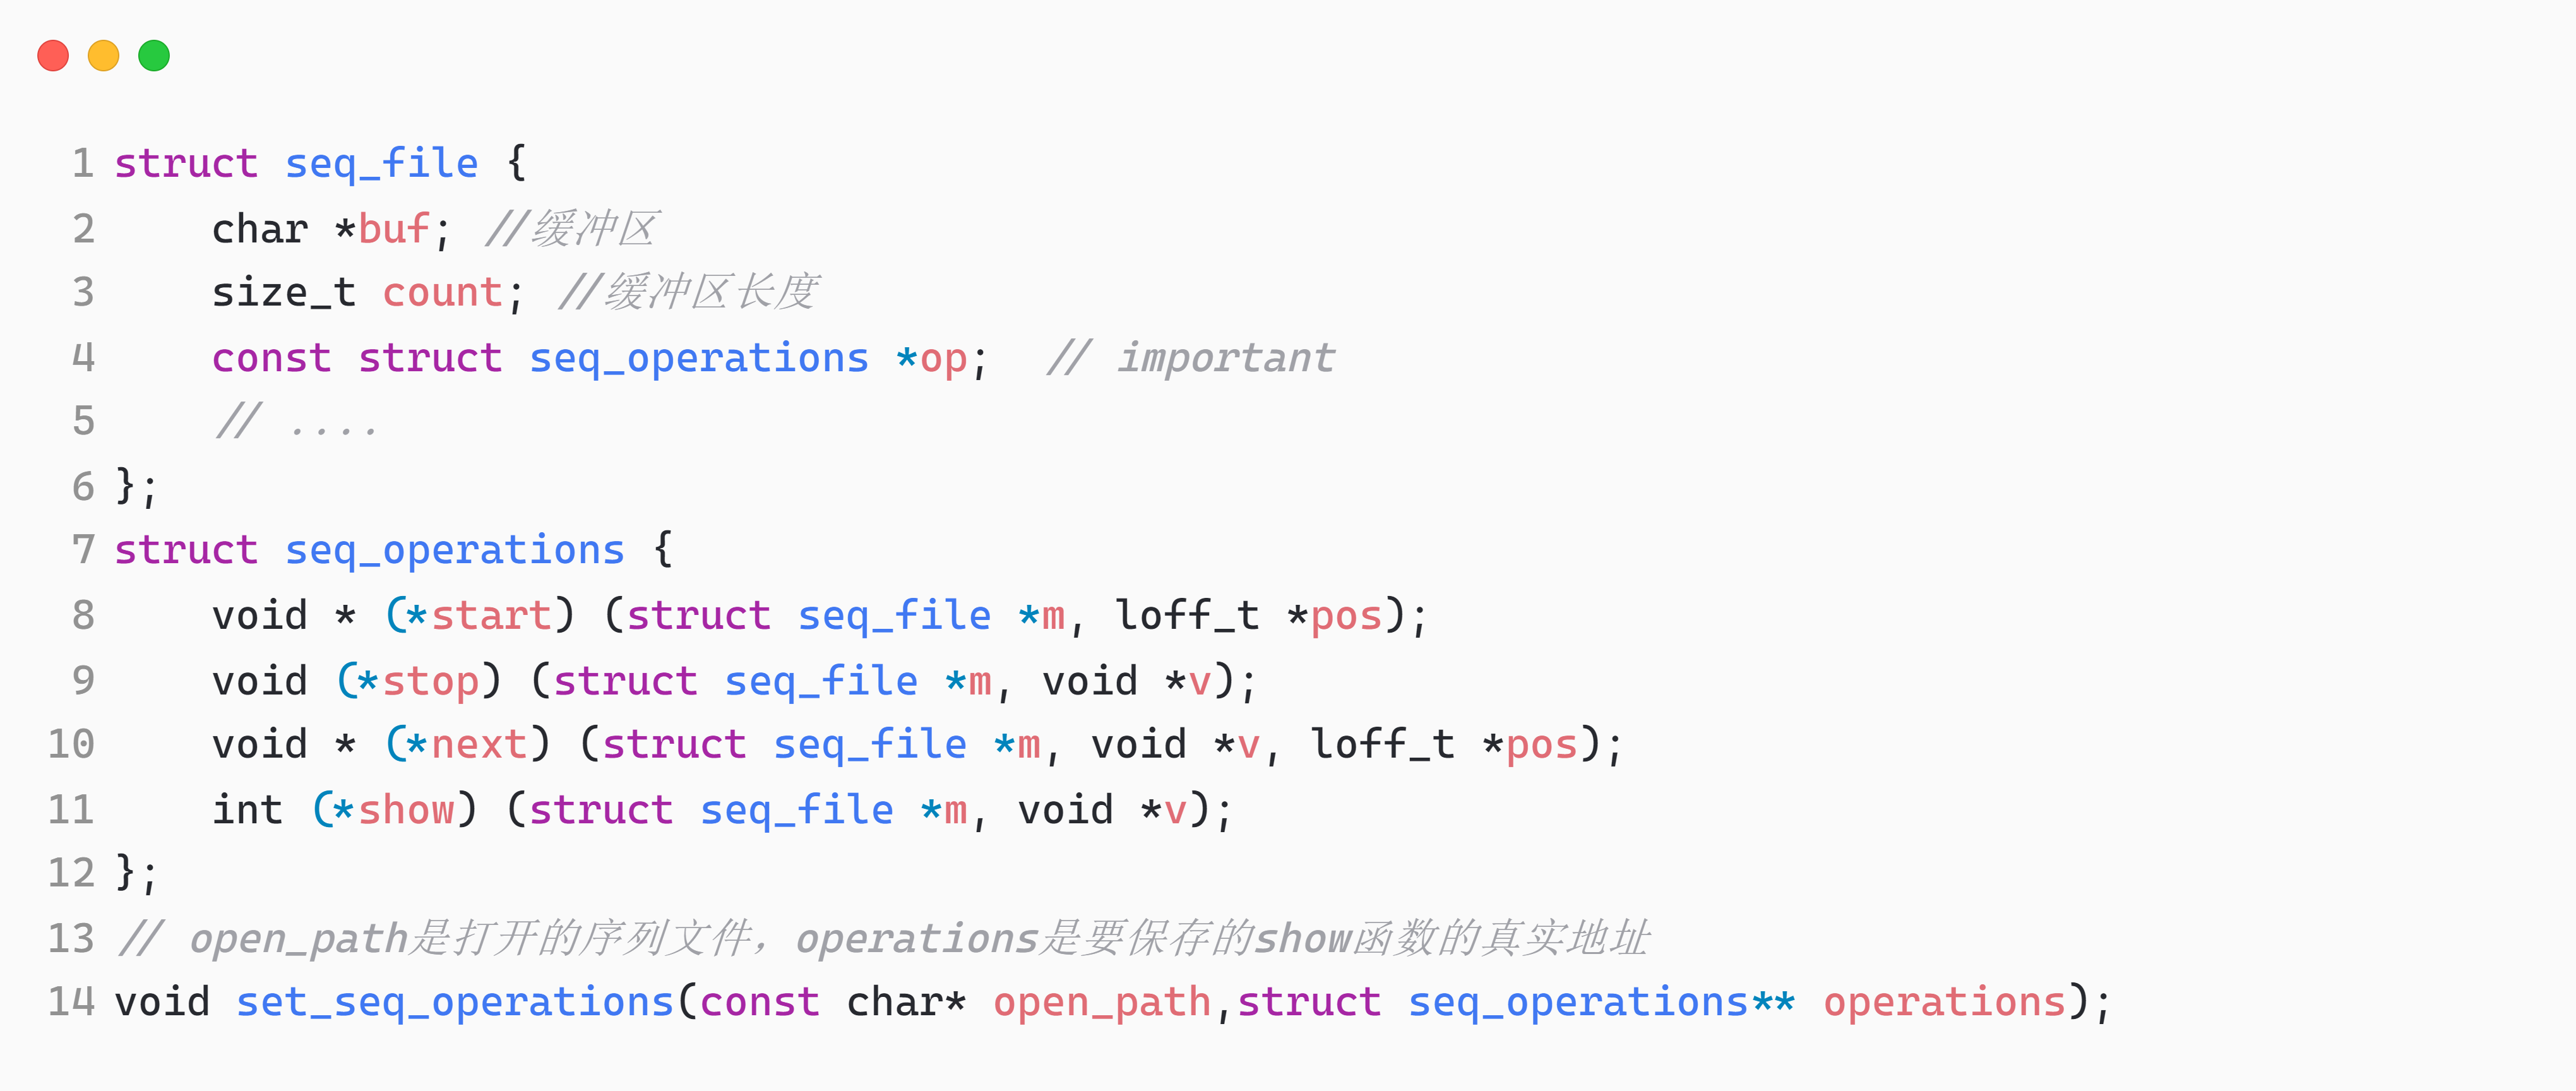
\includegraphics[width=0.95\textwidth]{pic/seq.png}
	\end{itemize}
\end{frame}

\begin{frame}
	\begin{itemize}
		\item hidden\_port\_list\_head存储要隐藏的端口
		\item hide\_connect函数将需要隐藏的端口添加到链表
		\item hide\_unconnect函数将该节点从链表中删除
		\item show函数会将需要展示的端口信息放在seq->buf中,而seq->count记录了buf的缓冲区长度
	\end{itemize}
	\begin{itemize}
		\centering
		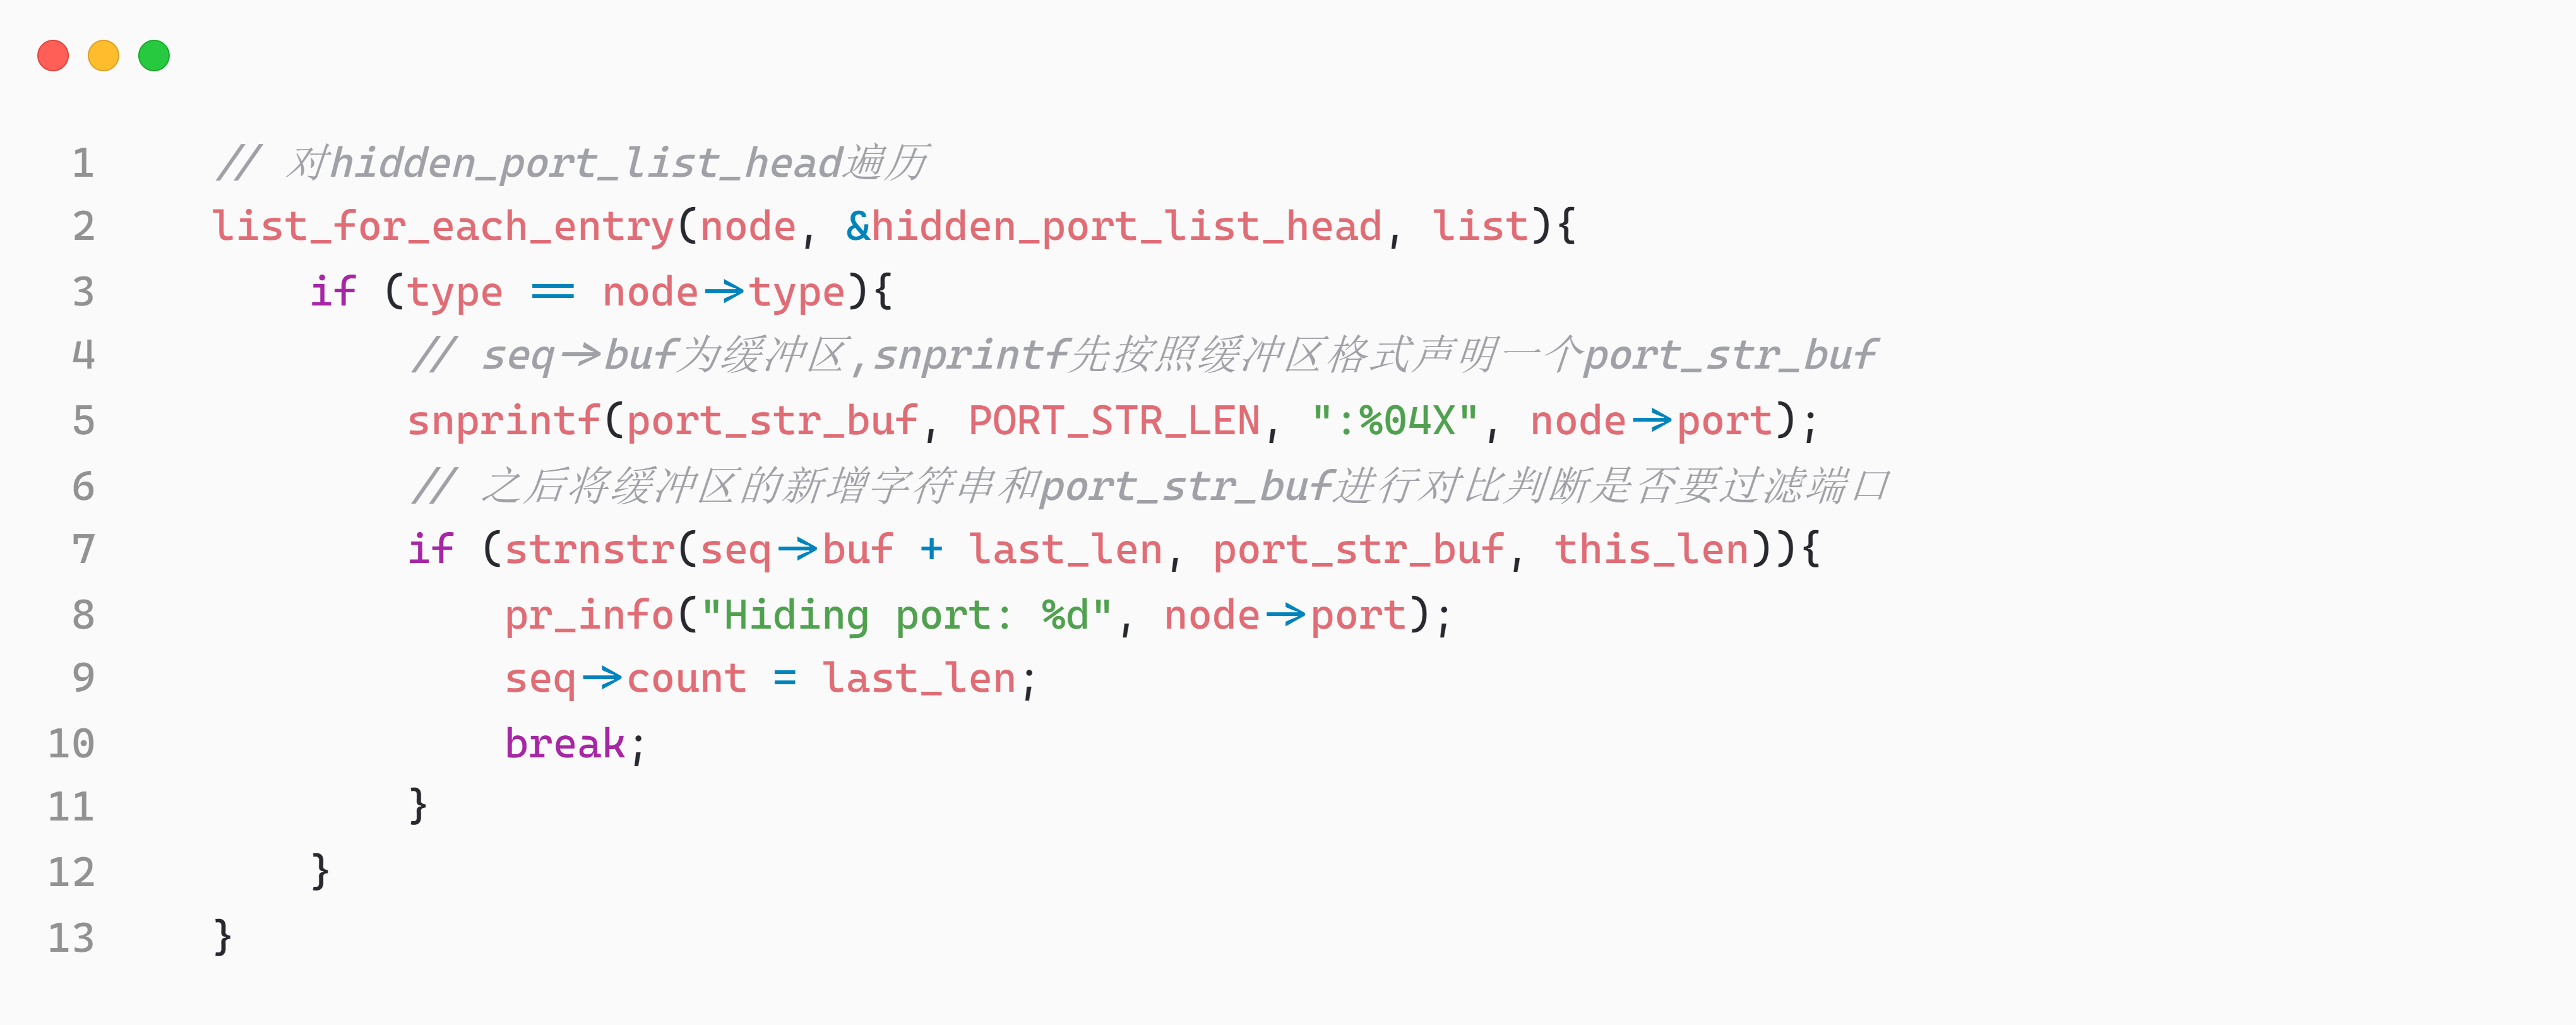
\includegraphics[width=0.95\textwidth]{pic/hideport.png}
	\end{itemize}
\end{frame}









%-------------------------------------------- 致谢
\begin{frame}
    \begin{center}
        {\Huge 感谢聆听与批评指正!}
    \end{center}
\end{frame}

\end{document}